\documentclass[10pt, a4paper]{report}
\usepackage[utf8]{inputenc}

\usepackage[T1]{fontenc}
\usepackage{hyperref}
\usepackage{natbib}
\usepackage[english, french]{babel}
\usepackage{graphicx}
\usepackage{fullpage}
\usepackage{eso-pic}
\usepackage{tcolorbox}
\usepackage{hyperref}
\usepackage[toc]{glossaries}
\usepackage{tikz}

\usepackage{listings}
\usepackage{background}
\usepackage{setspace}
\usepackage{titlepic}
\usepackage{booktabs} % Pour de jolis tableaux
\usepackage{tabularx} % Permet un ajustement automatique des colonnes
\usepackage[a4paper, top=2.5cm, bottom=2.5cm, left=3cm, right=2cm, margin=1in]{geometry} % Définit les marges pour éviter les débordements



% Définir les paramètres de l'image de fond pour la première page
\backgroundsetup{
	scale=2.5, % Échelle de l'image
	color=black, % Couleur de l'image (noir et blanc par défaut)
	opacity=0.1, % Opacité de l'image
	angle=0, % Angle de rotation de l'image
	position=current page.center, % Position de l'image centrée
	vshift=0cm, % Décalage vertical
	hshift=0cm, % Décalage horizontal
	contents={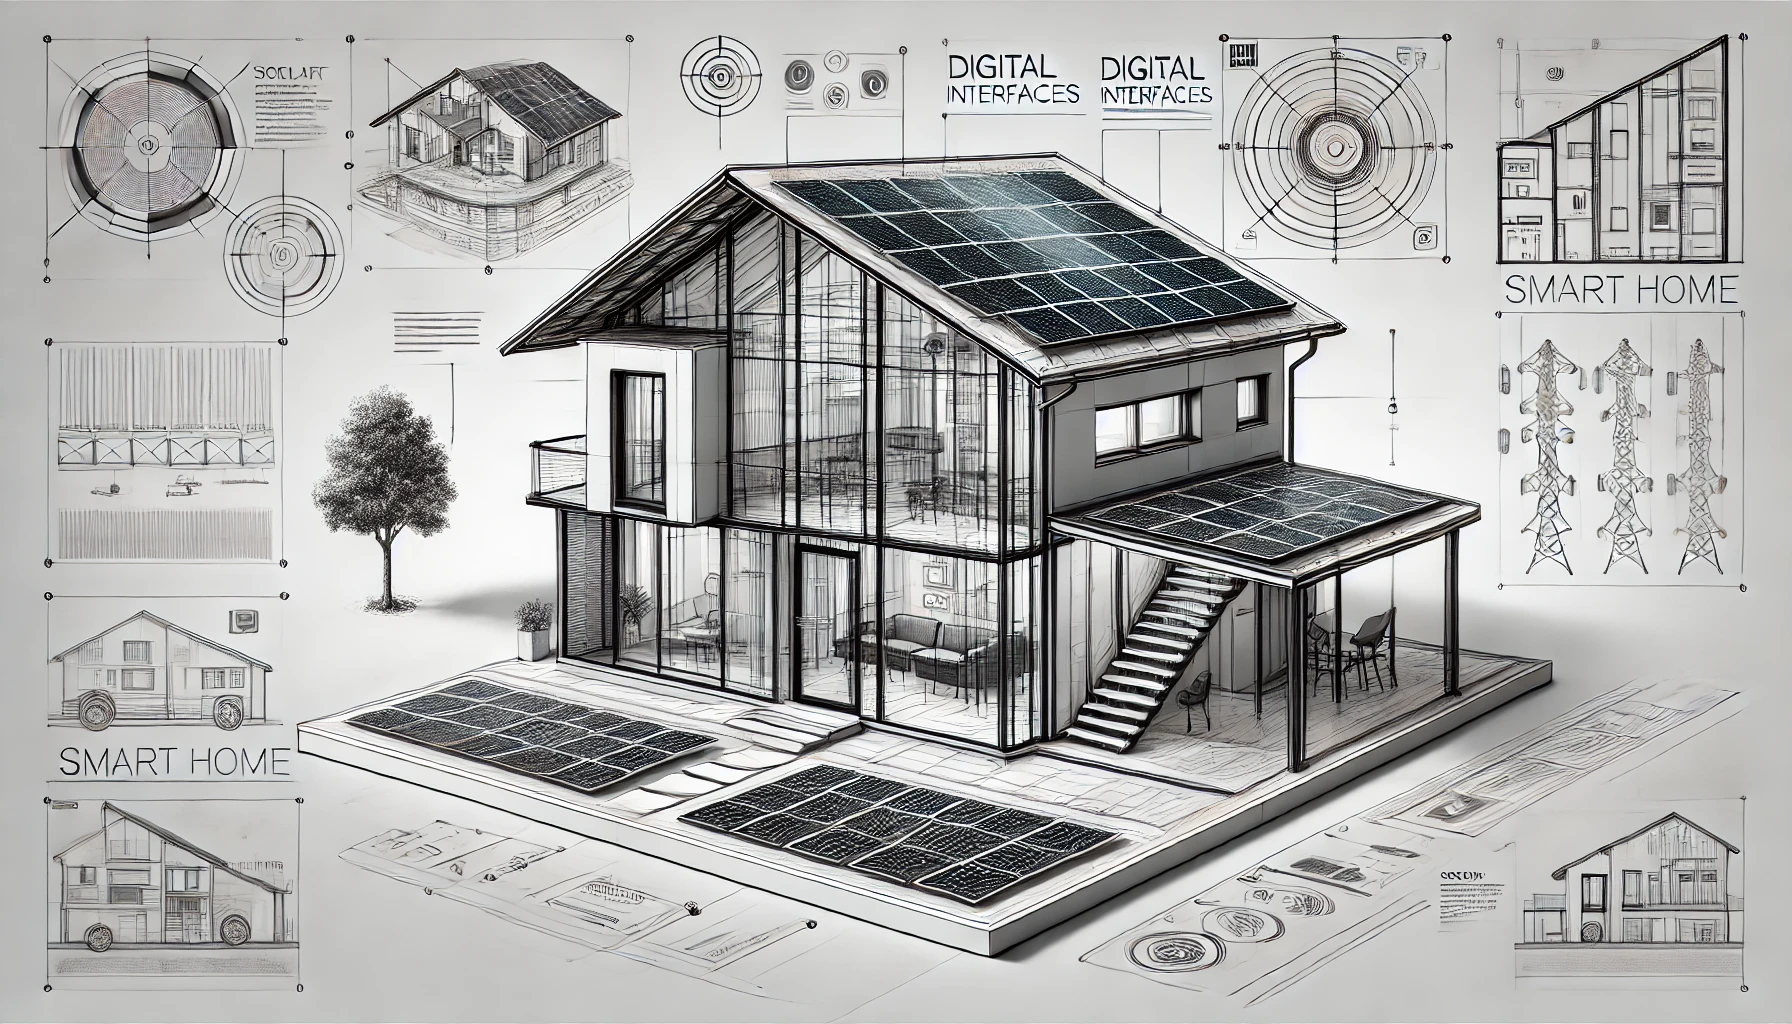
\includegraphics[width=\paperwidth]{ressources/img/logos/imageSmartHouse}} % Contenu (image de fond)
}


% Pour la lisibilité, on peut utiliser le package setspace pour ajuster l'espacement entre les lignes
\usepackage{setspace}
\usetikzlibrary{positioning, decorations.pathreplacing}

\definecolor{darkWhite}{rgb}{0.94,0.94,0.94}

\lstset{
	aboveskip=3mm,
	belowskip=-2mm,
	backgroundcolor=\color{darkWhite},
	basicstyle=\footnotesize,
	breakatwhitespace=false,
	breaklines=true,
	captionpos=b,
	commentstyle=\color{red},
	deletekeywords={...},
	escapeinside={\%*}{*)},
	extendedchars=true,
	framexleftmargin=16pt,
	framextopmargin=3pt,
	framexbottommargin=6pt,
	frame=tb,
	keepspaces=true,
	keywordstyle=\color{blue},
	language=Python,
	literate=
	{²}{{\textsuperscript{2}}}1
	{⁴}{{\textsuperscript{4}}}1
	{⁶}{{\textsuperscript{6}}}1
	{⁸}{{\textsuperscript{8}}}1
	{€}{{\euro{}}}1
	{é}{{\'e}}1
	{è}{{\`{e}}}1
	{ê}{{\^{e}}}1
	{ë}{{\¨{e}}}1
	{É}{{\'{E}}}1
	{Ê}{{\^{E}}}1
	{û}{{\^{u}}}1
	{ù}{{\`{u}}}1
	{â}{{\^{a}}}1
	{à}{{\`{a}}}1
	{á}{{\'{a}}}1
	{ã}{{\~{a}}}1
	{Á}{{\'{A}}}1
	{Â}{{\^{A}}}1
	{Ã}{{\~{A}}}1
	{ç}{{\c{c}}}1
	{Ç}{{\c{C}}}1
	{õ}{{\~{o}}}1
	{ó}{{\'{o}}}1
	{ô}{{\^{o}}}1
	{Õ}{{\~{O}}}1
	{Ó}{{\'{O}}}1
	{Ô}{{\^{O}}}1
	{î}{{\^{i}}}1
	{Î}{{\^{I}}}1
	{í}{{\'{i}}}1
	{Í}{{\~{Í}}}1,
	morekeywords={*,...},
	numbers=left,
	numbersep=10pt,
	numberstyle=\tiny\color{black},
	rulecolor=\color{black},
	showspaces=false,
	showstringspaces=false,
	showtabs=false,
	stepnumber=1,
	stringstyle=\color{gray},
	tabsize=4,
	title=\lstname,
}

% Additional language definitions
\lstdefinelanguage{JavaScript}{
	keywords={typeof, new, true, false, catch, function, return, null, catch, switch, var, if, in, while, do, else, case, break},
	keywordstyle=\color{blue}\bfseries,
	ndkeywords={class, export, boolean, throw, implements, import, this},
	ndkeywordstyle=\color{darkgray}\bfseries,
	identifierstyle=\color{black},
	sensitive=false,
	comment=[l]{//},
	morecomment=[s]{/*}{*/},
	commentstyle=\color{purple}\ttfamily,
	stringstyle=\color{orange}\ttfamily,
	morestring=[b]',
	morestring=[b]"
}

\lstdefinelanguage{C}{
	keywords={auto, break, case, const, continue, default, do, double, else, enum, extern, float, for, goto, if, inline, int, long, register, restrict, return, short, signed, sizeof, static, struct, switch, typedef, union, unsigned, void, volatile, while, _Bool, _Complex, _Imaginary},
	keywordstyle=\color{blue}\bfseries,
	identifierstyle=\color{black},
	sensitive=true,
	comment=[l]{//},
	morecomment=[s]{/*}{*/},
	commentstyle=\color{green}\ttfamily,
	stringstyle=\color{red}\ttfamily,
	morestring=[b]',
	morestring=[b]"
}

\makeglossaries
\newglossaryentry{API}
{
	name=API,
	description={(Interface de Programmation d'Application) est un ensemble de protocole permettant à différentes applications logicielle d'echanger des données entre elles}
}

\newcommand{\HRule}{\rule{\linewidth}{0.5mm}}
\newcommand{\blap}[1]{\vbox to 0pt{#1\vss}}
\newcommand\AtUpperLeftCorner[3]{%
	\put(\LenToUnit{#1},\LenToUnit{\dimexpr\paperheight-#2}){\blap{#3}}%
}
\newcommand\AtUpperRightCorner[3]{%
	\put(\LenToUnit{\dimexpr\paperwidth-#1},\LenToUnit{\dimexpr\paperheight-#2}){\blap{\llap{#3}}}%
}

\title{\LARGE{Smarthouse}}
\author{\textsc{Khedhaouria} Eliès \& \textsc{Marcelet} Paul}
\date{\today}
\makeatletter



\begin{document}
	\onehalfspacing % Définit l'espacement entre les lignes à 1.5
	
	
	\begin{titlepage}
		
		
		\enlargethispage{2cm}
		
		\AddToShipoutPicture{
			\AtUpperLeftCorner{1.5cm}{1cm}{
\includegraphics[width=6.5cm]{ressources/img/logos/isimaInp.png}}
		}
		
		\begin{center}
			\vspace*{10cm}
			
			\LARGE{\textbf{Rapport d'élève Ingénieur}}\\
			\LARGE{\textbf{Projet de troisième année}}\\
			\large{Filière:\textbf{ Sécurité} et \textbf{réseaux}} 
			\HRule
			\vspace*{0.5cm}
			\Huge{\textsc{\textbf{\@title}}}\\
			
		\end{center}
		\vspace*{2.5cm}
		Présenté par: \textbf{\@author }
		
		\vspace*{4.5cm}
		Responsable Isima: Monsieur \textbf{Alexandre GUITTON} \hspace*{2cm} Date de soutenance: \textbf{02/07/2024}\\\\
		\textbf{Campus des Cézeaux .  1 rue de la Chébarde .  TSA 60125 .  63178  Aubière CEDEX}
		
		
		
	\end{titlepage}
	\backgroundsetup{contents={}}
	\ClearShipoutPicture
	\newpage
	
	\tableofcontents
	\listoffigures
	
	\begin{abstract}
		\selectlanguage{french}
	Dans le cadre de notre projet de fin d’études, nous avons conçu et développé un \textbf{système de maison intelligente} 
	capable de transmettre \textbf{des données en temps réel de manière sécurisée} vers un serveur distant. L’objectif principal est de 
	mettre en place un \textbf{système de monitoring avancé}, permettant à un propriétaire de superviser et d’analyser les données 
	générées par ses équipements connectés.
	
	Pour garantir \textbf{l’intégrité et la confidentialité des échanges}, nous avons implémenté une \textbf{communication sécurisée 
	basée sur des certificats SSL/TLS} et le protocole \textbf{MQTTs}, assurant ainsi une transmission chiffrée et authentifiée entre 
	la maison et le serveur.
	
	Les données collectées par les capteurs sont stockées dans une \textbf{base de données à série temporelle} (InfluxDB), 
	spécialement optimisée pour le traitement et l’analyse de données en flux continu.
	
	Une \textbf{API centralisée}, développée en \textbf{Laravel}, a été mise en place afin de :
	\begin{itemize}
		\item \textbf{gérer la création des propriétaires} et l’association sécurisée de leurs équipements.
		\item \textbf{automatiser la génération et la signature des certificats} pour garantir une authentification fiable.
		\item \textbf{offrir une interface d’accès aux données}, permettant aux utilisateurs de récupérer \textbf{des données en temps 
		réel ou historiques}, selon différents filtres appliqués à la base de données.
	\end{itemize}
	
	Enfin, une \textbf{interface graphique interactive}, développée en \textbf{Qt}, permet aux utilisateurs de \textbf{visualiser les 
	données en temps réel} sous forme de \textbf{graphiques dynamiques}. Cette interface interagit directement avec l’API afin de 
	récupérer et d’afficher \textbf{les données filtrées}, qu’elles soient en temps réel ou issues d’une période spécifique dans le 
	passé.
	
	Ce projet intègre \textbf{des technologies modernes et des concepts avancés en sécurité, IoT, gestion des bases de données et 
	visualisation de données en temps réel}, assurant ainsi une \textbf{infrastructure robuste, fiable et évolutive}.

	\end{abstract}
	\selectlanguage{english}
	\begin{abstract}
		As part of our final-year engineering project, we designed and developed a \textbf{smart home system} capable of 
		securely transmitting \textbf{real-time data} to a remote server. The main objective is to implement an \textbf{advanced 
		monitoring system} that allows a homeowner to monitor and analyze data generated by their connected devices.
		
		To ensure \textbf{data integrity and confidentiality}, we implemented a \textbf{secure communication protocol based on SSL/TLS 
		certificates} and the \textbf{MQTTs protocol}, providing encrypted and authenticated communication between the home and the 
		server.
		
		Sensor data is stored in a \textbf{time-series database} (InfluxDB), optimized for real-time data processing and analysis.
		
		A \textbf{centralized API}, developed in \textbf{Laravel}, has been implemented to:
		\begin{itemize}
			\item \textbf{Manage the creation of homeowners} and the secure association of their devices.
			\item \textbf{Automate the generation and signing of certificates} to ensure reliable authentication.
			\item \textbf{Provide a data access interface}, allowing users to retrieve \textbf{real-time or historical data} based on 
			various filters applied to the database.
		\end{itemize}
		
		Finally, an \textbf{interactive graphical interface}, developed in \textbf{Qt}, allows users to \textbf{visualize real-time 
		data} using \textbf{dynamic graphs}. This interface directly interacts with the API to retrieve and display \textbf{filtered 
		data}, whether in real-time or from a specific historical period.
		
		This project integrates \textbf{modern technologies and advanced concepts in security, IoT, database management, and real-time 
		data visualization}, ensuring a \textbf{robust, reliable, and scalable infrastructure}.
		
	\end{abstract}
	
	
	\chapter{Introduction}
		La \textbf{domotique} représente aujourd'hui un enjeu majeur dans le domaine des innovations technologiques. Avec l'essor des 
		\textbf{maisons connectées} et des \textbf{IOTs}, les utilisateurs peuvent désormais \textbf{surveiller} et \textbf{contrôler} 
		leur domicile à distance, leur assurant ainsi une amélioration significative en termes de \textbf{sécurité}, 
		\textbf{d'efficacité énérgétique} et de \textbf{confort}. Cette évolution s'inscrit dans un contexte plus large dans lequel 
		l'automatisation et la connectivité jouent un rôle crucial dans notre quotidien.\\
		Le \textbf{monitoring à distance} des équipements d'une maison constitue un axe fondamental de la domotique moderne. Il permet 
		aux propriétaires d'obtenir une \textbf{vue globale de l'état de leur habitation en temps réel}. Cela joue un rôle crucial dans 
		plusieurs domaines:
		\begin{itemize}
			\item il permet de \textbf{sécuriser} un domicile, permettant par exemple la détéction d'intrusion ainsi que la prévention 
			des cambriolages
			
			\item il \textbf{optimise énergiquement} le domicile, par le biais de l'automatisation des objets 
			connectés, en fonction d'horaires programmés, afin d'optimiser la consommation d'énergie.
			
			\item et il permet enfin \textbf{un confort et un contrôle à distance}, offrant aux propriétaires la possibilité d'activer ou 
			de désactiver certains dispositifs sans être physiquement présent.\\
		\end{itemize}
		Si ces avancées technologiques offrent des opportunités considérables, elles soulèvent néanmoins une problématique critique: 
		\textbf{la sécurisation des dispositifs IoTs et du transfert des données}. Aujourd'hui, de nombreux objets connectés sont 
		déployés avec des failles de sécurité importantes souvent négligées par les fabricants et les utilisateurs. Des outils comme 
		\textbf{Shodan}, un moteur de recherche spécialisé dans l'identification des appareils connectés exposés sur Internet, mettent 
		en évidence la vulnérabilité de nombreux systèmes IoTs accessibles sans protection adéquate. Cette situation constitue un risque 
		majeur, rendant possible des cyberattaques capables de compromettre \textbf{l'intégrité} et \textbf{la confidentialité} des 
		données échangées.\\
		Ce rapport décrit une architecture, solution à cette problématique en explorant l'une des applications majeures de la domotique: 
		\textbf{le monitoring à distance des capteurs d'une maison connectée, ainsi que l'établissement d'une communication sécurisée et 
		authentifiée entre celle-ci et un serveur distant}. L'objectif est de permettre aux utilisateurs de récupérer des \textbf{données 
		en temps réel}, issues de capteurs de leur domicile tout en garantissant \textbf{une transmission chiffrée} afin de protéger les 
		échanges contre d'éventuelles interceptions malveillantes. C'est à partir de cela que l'on peut définir une problématique à 
		laquelle la solution doit répondre: \textbf{Comment développer un système de monitoring en temps réel pour une maison connectée, 
		garantissant la sécurité de la transmission des données tout en renforcant l'authentification des équipements IoTs ?}
		
	
	\chapter{Contexte du Projet}
	\section{Analyse du besoin et définition des objectifs}
		Lorsqu'un résident quitte son domicile, il peut être préoccupé par l'état de sa maison, se demandant si une lumière a bien été éteinte ou si une fenêtre a été correctement fermée. Ces préoccupations sont légitimes, d'autant plus que les statistiques récentes indiquent une augmentation des cambriolages des logements en France. En effet au 30 juin 2024, les forces de sécurité ont enregistré une hausse de 4\% des cambriolages de logements sur les douze derniers mois\footnote{source: \url{https://www.interieur.gouv.fr/actualites/actualites-du-ministere/analyse-conjoncturelle-des-crimes-et-delits-enregistres-par} et \url{https://mobile.interieur.gouv.fr/Interstats/Actualites/Info-Rapide-n-43-La-delinquance-enregistree-par-la-police-et-la-gendarmerie-nationales-un-point-a-mi-annee-2024}}. Cette tendance souligne la nécessité de renforcer les dispositifs de sécurité pour protéger les habitations.\\
		Parallèlement, la proliférations des dispositifs IOT dans les foyers pose des défis non négligeables en matière de cybersécurité. Bien que ces technologies offrent des avantages indéniables en termes de confort et d'efficacité énergetiques, elles peuvent constituer des points d'entrée pour les cybercriminelles si elles ne sont pas correctement sécurisées. Il est ainsi essentiel de garantir que seuls les propriétaires autorisés aient accès à ces dispositifs et que les données transmises soient protégées contre toute altération ou interception malveillante.\\
		Fâce à ces constats, notre projet vise à développer une solution permettant la transimission sécurisée issues de capteurs IoTs d'une maison vers un serveur distant. Cette solution devra assurer l'authentification des dispositifs, garantir l'intégrité ainsi que la confidentialité des données, et ainsi permettre aux propriétaires de surveiller à distance l'état de leur domicile en temps réel.
	\section{Organisation de la conception à la création}
	Dans le cadre du développement de ce projet, nous avons adopté une approche structurée en plusieurs phases allant de la simulation initiale de l'environnement domotique jusqu'à la mise en place d'une infrastructure de communication sécurisée et fiable.\\\\
	\textbf{Phase 1: Simulation de l'environnement domotique et émission des données}\\
	Avant de mettre en place l'architecture réseau et serveur, nous avons débuté par la simulation logicielle de la maison connectée, en programmant un environnement permettant la génération de données de divers capteurs (température, humidité, lumière...). Cette simulation développée en \textbf{Python}, modélise une maison contenant divers équipements Iots et capteurs, emettant des séries de données à temps réel.\\
	L'objectif principal de cette étape était de tester l'envoie de séries de données, à intervalle régulier, au sein d'un serveur distant (Phase suivante), en utilisant le protocole de communication \textbf{MQTT}. À ce moment là, la transmission s'effectuait sans authentification ni chiffrement, nous permettant ainsi, de valider l'intégralité du transport, la récéption au serveur et d'évaluer aussi les performances du protocole. \\\\
	\textbf{Phase 2: Mise en place de l'infrastructure serveur}\\
	Une fois la simulation fonctionnelle, nous avons déployé une \textbf{infrastructure serveur} sous une machine virtuelle \textbf{Ubuntu}, utilisant l'hyperviseur \textbf{Virtualbox} avec un accès par pont en configuration réseau. Ce serveur assure le rôle de récépteur des données envoyées par la maison connectée.\\
	Afin de permettre la récéption ainsi que le sotckage des données, nous avons mis en place plusieurs composants essentiels:\\
	\begin{itemize}
		\item \textbf{Mosquitto}: Un broker \textbf{MQTT} permettant la gestion des messages entre les maisons connectées et le serveur aux divers topics.
		\item \textbf{InfluxDB}: Une \textbf{base de données à séries temporelles}, choisie pour sa capacité à stocker et traiter efficacement des flux de données en temps réel.
		\item \textbf{Telegraf}: Un agent de collecte des données utilisé pour formaliser et structurer les données reçues depuis le \textbf{Broker} avant leur insertion dans la base de données.\\
	\end{itemize}
	À la fin de cette étape, après configuration des composants, l’infrastructure était fonctionnelle, mais vulnérable : les données envoyées par les capteurs n’étaient pas protégées et n’importe quel utilisateur pouvait intercepter ou publier des messages MQTT sur le serveur, compromettant ainsi l’intégrité du système.\\\\
	\textbf{Phase 3: Sécurisation des échanges et authentifications des Maisons}\\
	Afin de garantir l'\textbf{authenticité des émetteurs} et de protéger les données échangées, nous avons implémenté une \textbf{authentification basée sur des certificats SSL/TLS} pour le protocole MQTT. Cette sécurisation repose sur \textbf{l'utilisation de certificats clients} générés par une autorité de certifcation interne au serveur, exigeant une \textbf{authentification mutuelle} entre la maison et le serveur pour toute communication MQTT ainsi que le \textbf{chiffrement des échanges} grâce à TLS qui empêche toute interception des données transmises.\\
	Ce mécanisme permet ainsi de \textbf{garantir l'identité des dispositifs connectés} et d'empêcher ainsi toute inteception des données par un acteur non autorisé.\\\\
	\textbf{Phase 4 : Développement d’une API centralisant l’accès aux données}\\
	Afin de faciliter l'accès aux données, d'éviter une exposition directe du broker MQTT et aussi de permettre par la suite la création d'interfaces fonctionnant sur divers plateformes, nous avons développé une \textbf{API Rest sous Laravel}, jouant deux rôles importants:\\
	\begin{itemize}
		\item \textbf{Gestion de propriétaires et authentification:} l'API permet la \textbf{création de propriétaires} assurant une authentification unique et sécurisée. Un nouvel utilisateur peut en effet s'enregistrer en tant que propriétaire, l'API lui générera ainsi un \textbf{token unique}, qui servira \textbf{d'identifiant primaire} pour toutes les interactions futures entre les propriétés de l'utilisateur et le système. Elle générera de plus, un \textbf{certificat client signé} par l'autorité de certification accompagné d'une clé privée, permettant ainsi une authentification sécurisée lors des échanges avec le broker MQTT.
		
		\item \textbf{API de relais et récupération des données: } l'API agit également en tant que \textbf{relais sécurisé} entre les propriétaires et les données stockées au sein du serveur. L'API est capable d'extraire les series temporelles stockées au sein de \textbf{InfluxDB}, en les filtrant en fonction des critères demandés pour chaque utilisateurs (temps réel, historique...). Ainsi, les utilisateurs peuvent accéder uniquement aux données qui leur sont déstinées, garantissant l'intégrité et la confidentialité des échanges.\\
	\end{itemize}
	 
	
	\textbf{Phase 5: Développement d'une interface graphique  permettant un affichage concret des données}
	
	Afin de permettre une visualisation claire des données issues des capteurs, nous avons eu l'idée de développer une interface graphique utilisant \textbf{Qt}. Cette interface permet aux propriétaires d'interagir avec l'\textbf{API}
	et d'accéder aux informations de leur maison de manière ergonomique.\\
	Le but de l'interface QT est de récupérer les données via l'API en appliquant divers critères de filtrage, et placer les résultats affichés sous forme de graphique dynamique, afin de faciliter l'analyse ainsi que la supervision de la maison connectée.\\
	Le choix d'utiliser Qt comme technologie, est liée à plusieurs raisons:\\
	\begin{itemize}
		\item \textbf{Demande élevée en entreprise: } Qt est largement utilisé dans l’industrie pour le développement d’interfaces utilisateur performantes et multiplateformes.
		\item \textbf{Complémentarité avec les connaissances acquises en C++:} jusqu’à présent, le programme de formation avait principalement abordé le C++ de manière théorique. Ce projet était donc une opportunité idéale pour appliquer concrètement ses connaissances en développant une interface interactive et fonctionnelle.
	\end{itemize}
	\vspace{3cm}
	\begin{figure}[h!]
		\centering
		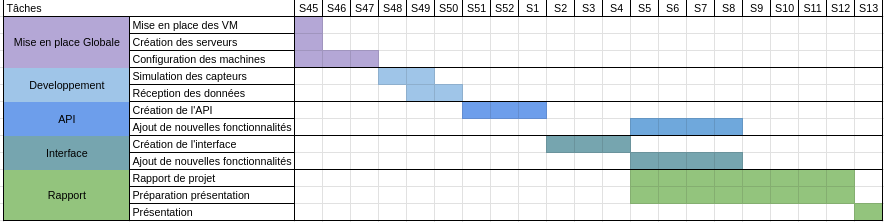
\includegraphics[width=1\textwidth]{ressources/img/Gantt/diagrammePrevisionnel}
		\caption{Diagramme de Gantt \textbf{Prévisionnel}}
		\label{fig:GanttPrevisionnel}
	\end{figure}
		\begin{figure}[h!]
		\centering
		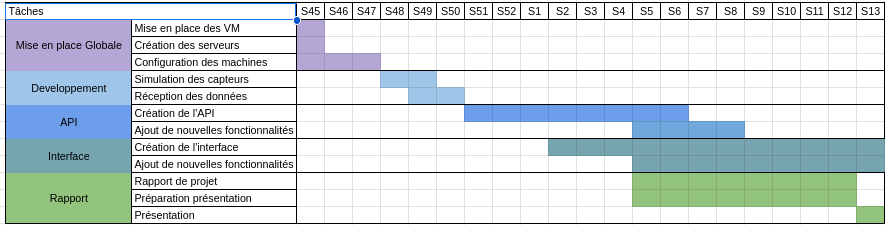
\includegraphics[width=1\textwidth]{ressources/img/Gantt/diagrammeReel}
		\caption{Diagramme de Gantt \textbf{réel}}
		\label{fig:GanttReel}
	\end{figure}
	
	
	\chapter{Conception et Implémentation}
	
	\section{Infrastructure et Environnement de Développement}
	Cette section détaille l'ensemble de l’infrastructure mise en place, depuis la simulation logicielle d'une maison connectée jusqu'à l'infrastructure serveur dédiée. Cette dernière assure la \textbf{réception}, le \textbf{traitement} ainsi que le \textbf{stockage} sécurisé des données issues des différents capteurs IoT simulés. Nous présenterons les diverses technologies utilisées au sein de l'infrastructure, ainsi que la façon dont elles ont été intégrées afin de garantir une cohérence globale avec les objectifs initiales du projet.\\
	Ce projet a été réalisé en \textbf{local}, sous la forme d'une \textbf{simulation globale}. Le serveur utilisé repose sur une machine virtuelle exécutant \textbf{Ubuntu Server}, configurée localement via \textbf{un accès réseau en mode pont}. Cette configuration permet au serveur d'obtenir une adresse IP dédiée sur le même réseau local que la machine hôte, facilitant ainsi une connectivité réseau directe et simplifiée avec la maison connectée simulée. Dans ce contexte, notre simulation considère que le serveur et l’émetteur sont présents au sein du même réseau local, en l'absence de solution Cloud externe.\\
	Nous verrons que le serveur joue un rôle central au sein de cette infrastructure. En effet, il héberge l'ensemble des services essentiels au fonctionnement de la solution réceptrice: le \textbf{broker MQTT}, l'\textbf{API REST} développée sous Laravel, ainsi que l'ensemble des bases de données qu'elles soient à\textbf{ séries temporelles ou relationnelles}.\\
	Concernant l'infrastructure émettrice, afin de simuler les équipement IOTs de la \textbf{maison connectée}, nous avons utilisé le\textbf{ language Python} du fait de la disponibilité étendue des bibliothèques réseau faciles à implémenter, facilitant ainsi la mise en œuvre rapide et fiable de la simulation. \\
	Dans les sous-sections suivantes, nous détaillerons la mise en place précise de chacun des composants techniques essentiels à la réalisation de nos objectifs.
		\begin{figure}[h!]
		\centering
		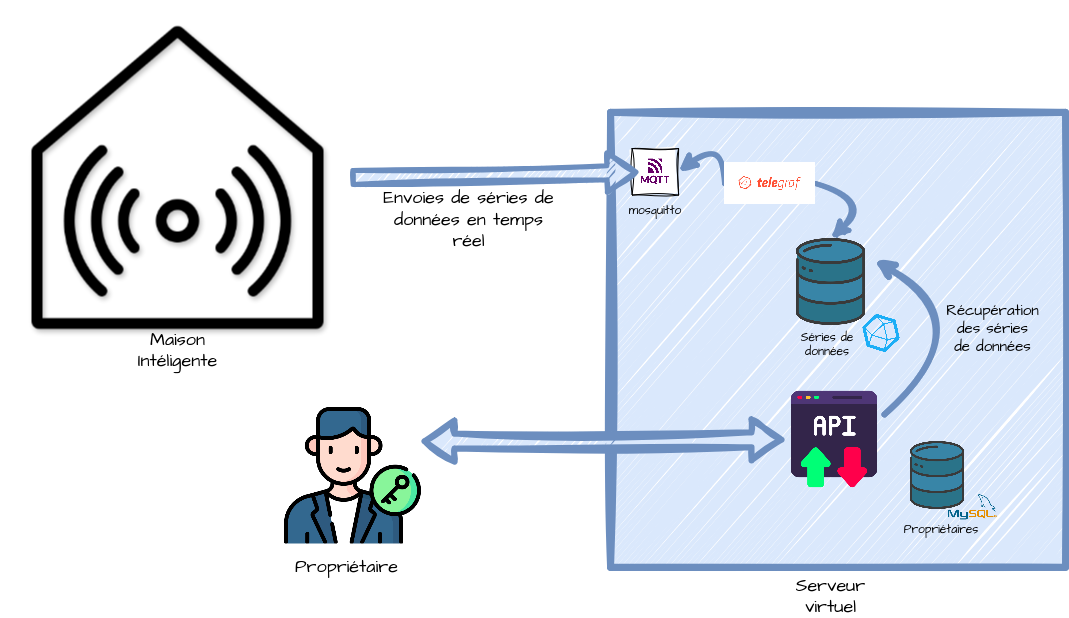
\includegraphics[width=0.5\textwidth]{ressources/img/shémas/shemaInfras.png}
		\caption{Architecture de l'infrastructure fonctionnelle}
		\label{fig:archiInfra}
	\end{figure}
	
	Le schéma ci-dessus décrit l'infrastructure globale mis en place au sein de la section.
	
	
 
	\subsection{Simulation du serveur et architecture réseau}
	\subsubsection{Déploiement d'un Broker MQTT sécurisé}
	
	Afin de garantir une transmission en temps réel des données IoTs entre la maison connectée et le serveur, nous avons trouver plus judicieux de choisir le protocole \textbf{MQTT}.\\
	\textbf{MQTT} est un protocole de messagerie léger basé sur le modèle \textbf{publish/subscribe}, initialement conçu pour des environnements où la bande passante est limitée et la latence est faible. MQTT est, dans notre contexte, parfaitement adapté. En effet, le protocole a initialement été concu afin d'être adapté aux applications IoTs, grâce à sa faible consommation de ressources, sa simplicité d'implémentation et son support pour des communications asynchrones et pouvant être sécurisées par le biais de la technologie \textbf{SSL/TLS}.\\\\
	Il est important de savoir que MQTT repose sur trois éléments fondamentaux:
	\begin{itemize}
		\item \textbf{le Broker (serveur de message):} Element central de l'architecture MQTT agissant comme un relais entre les clients acheminant les messages publiés et les abonnés appropriés. Il en existe un certain nombre, et dans le cadre de notre projet, nous avons choisi d'utiliser \textbf{Mosquitto}.
		
		\item \textbf{les Topics (Sujets de message):} Il s'agit d'une chaîne hierarchique permettant d'identifier une catégorie de messages, leur format est composé de "/" permettant de séparrer les sous-topics. Dans le cadre de notre projet nous avons justement exploité ce système de chaînes hiérarchiques afin d'organiser d'une manière précise, l'ensemble des types d'\textbf{iots} situés dans les différentes salles des divers \textbf{maisons} des différents \textbf{propriétaires}. 
		
		\item \textbf{les clients (publishers et subscribers):} MQTT fait la distinction entre deux types de clients: 
		\begin{itemize}
			\item \textbf{les pusblishers (éditeurs)}, ceux qui envoient des messages à un topic spécifique, sans se soucier du destinataire, il s'agit dans le cadre de notre projet, de la \textbf{maison connectée} qui envoie des series de données aux différents topics correspondants. 
			
			\item \textbf{les subscribers (abonnés)} ceux qui écoutent au sein d'un topic et reçoivent les messages spécifiques correspondants, dans notre cas, il s'agit des \textbf{propriétaires} des maisons.
		\end{itemize}
	\end{itemize}
	\vspace{0.5cm}
	
	Tel qu'expliqué, nous avons choisis de déployer \textbf{Mosquitto} au sein du serveur. Malgré le fait qu'il existe d'autres solutions telles que \textbf{HiveMQT}, \textbf{EMQX} ou \textbf{RabbitMQ MQTT}, pouvant faire office de \textbf{broker}, nous avons choisit \textbf{Mosquitto}, du fait qu'il est conçu pour être \textbf{ultra-léger}, consommer \textbf{très peu de mémoire et de CPU même sous forte charge}, et convient aussi bien \textbf{aux petits réseaux IoT qu'aux grandes infrastructures}.\\
	De plus, \textbf{Mosquitto} permet une installation assez rapide de son service, et la configuration s'effectue via un seul fichier : \textbf{mosquitto.conf}. Enfin, il supporte des fonctionnalités de sécurité avancées que nous avons mis en place au sein de notre serveur, telles que le support \textbf{TLS/SSL} afin de chiffrer les communications.\\
	Pour sécuriser les connexions et assurer l'authenticité des communications, nous avons implémenté MQTT sécurisé (MQTTs) basé sur SSL/TLS. Nous avons utilisé l’outil \textbf{OpenSSL} pour créer une autorité de certification interne \textbf{CA} ainsi que pour \textbf{générer et signer automatiquement} des certificats clients \textbf{client.crt} et leurs clés privées associées \textbf{client.key}. Chaque maison simulée dispose donc de trois certificats essentiels pour établir une connexion sécurisée.\\\\
	Voici ainsi l'architecture de sécurisation de \textbf{Mosquitto}:
	\begin{itemize}
		 \item la création d'une Autorité de Certification (CA) dédiée pour la \textbf{génération et la signature des certificats}.
		\item l'utilisation de certificats clients signés (certificat client et clé privée) pour chaque maison voulant envoyer des données au sein d'un serveur.
		\item l'utilisation du protocole MQTTs, permettant une \textbf{authentification mutuelle} et un chiffrement systématique des communications, empêchant ainsi toute interception ou injection malveillante de données.
	\end{itemize}
	
	\vspace{1cm}
	
	Pour faciliter la compréhension de la sécurisation de Mosquitto, et l'intégration du protocole MQTTs au sein de l'architecture, voici un schéma explicatif: 
	\begin{figure}[h!]
		\centering
		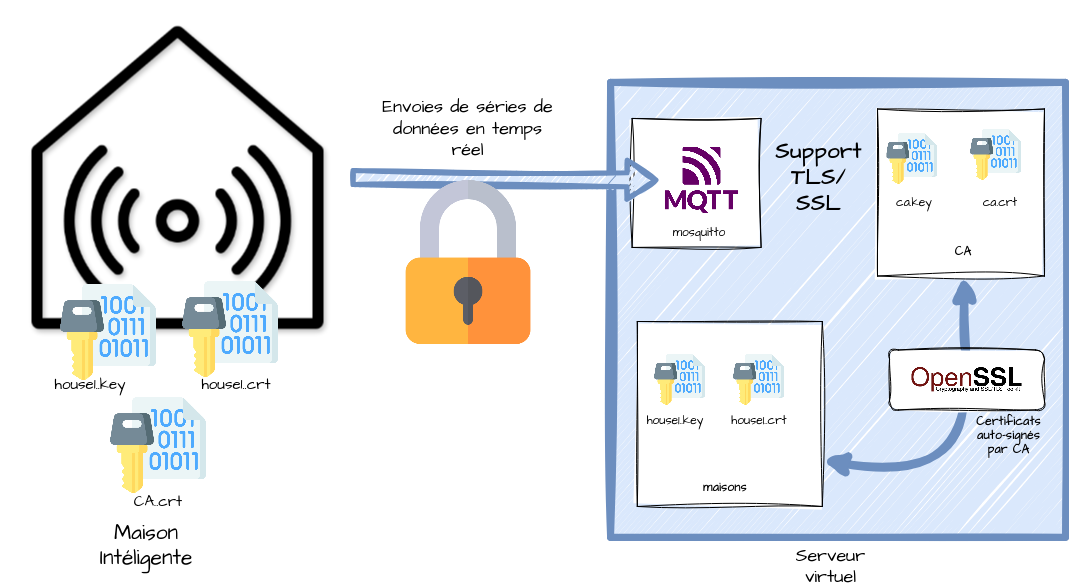
\includegraphics[width=0.5\textwidth]{ressources/img/shémas/shemaEmissionSSL.drawio.png}
		\caption{Sécurisation de mosquitto}
		\label{fig:secuMosquitto}
	\end{figure}
	
	Afin de vérifier le fonctionnement des certificats ainsi que l'envoi de données au sein du broker mosquitto du serveur virtuel, nous avons à ce moment là testé avec les commandes \textbf{mosquitto\_pub côté client} et les \textbf{logs temps réel côté serveur}\footnote{Au sein de la configuration de mosquitto, nous avons définit un chemin de log accessible en temps réel via la commande linux \textbf{tail -f /var/log/mosquitto/mosquitto.log}}.\\\\ Ainsi, après génération et auto-signature des certificats, les figures ci-dessous montrent ce qu'il se passe lorsque l'authentification est valide c'est à dire lorsque le \textbf{client.key} et le \textbf{client.crt} correspondent bien, et lorsque ces derniers sont invalides:
	
	\begin{figure}[h!]
		\centering
		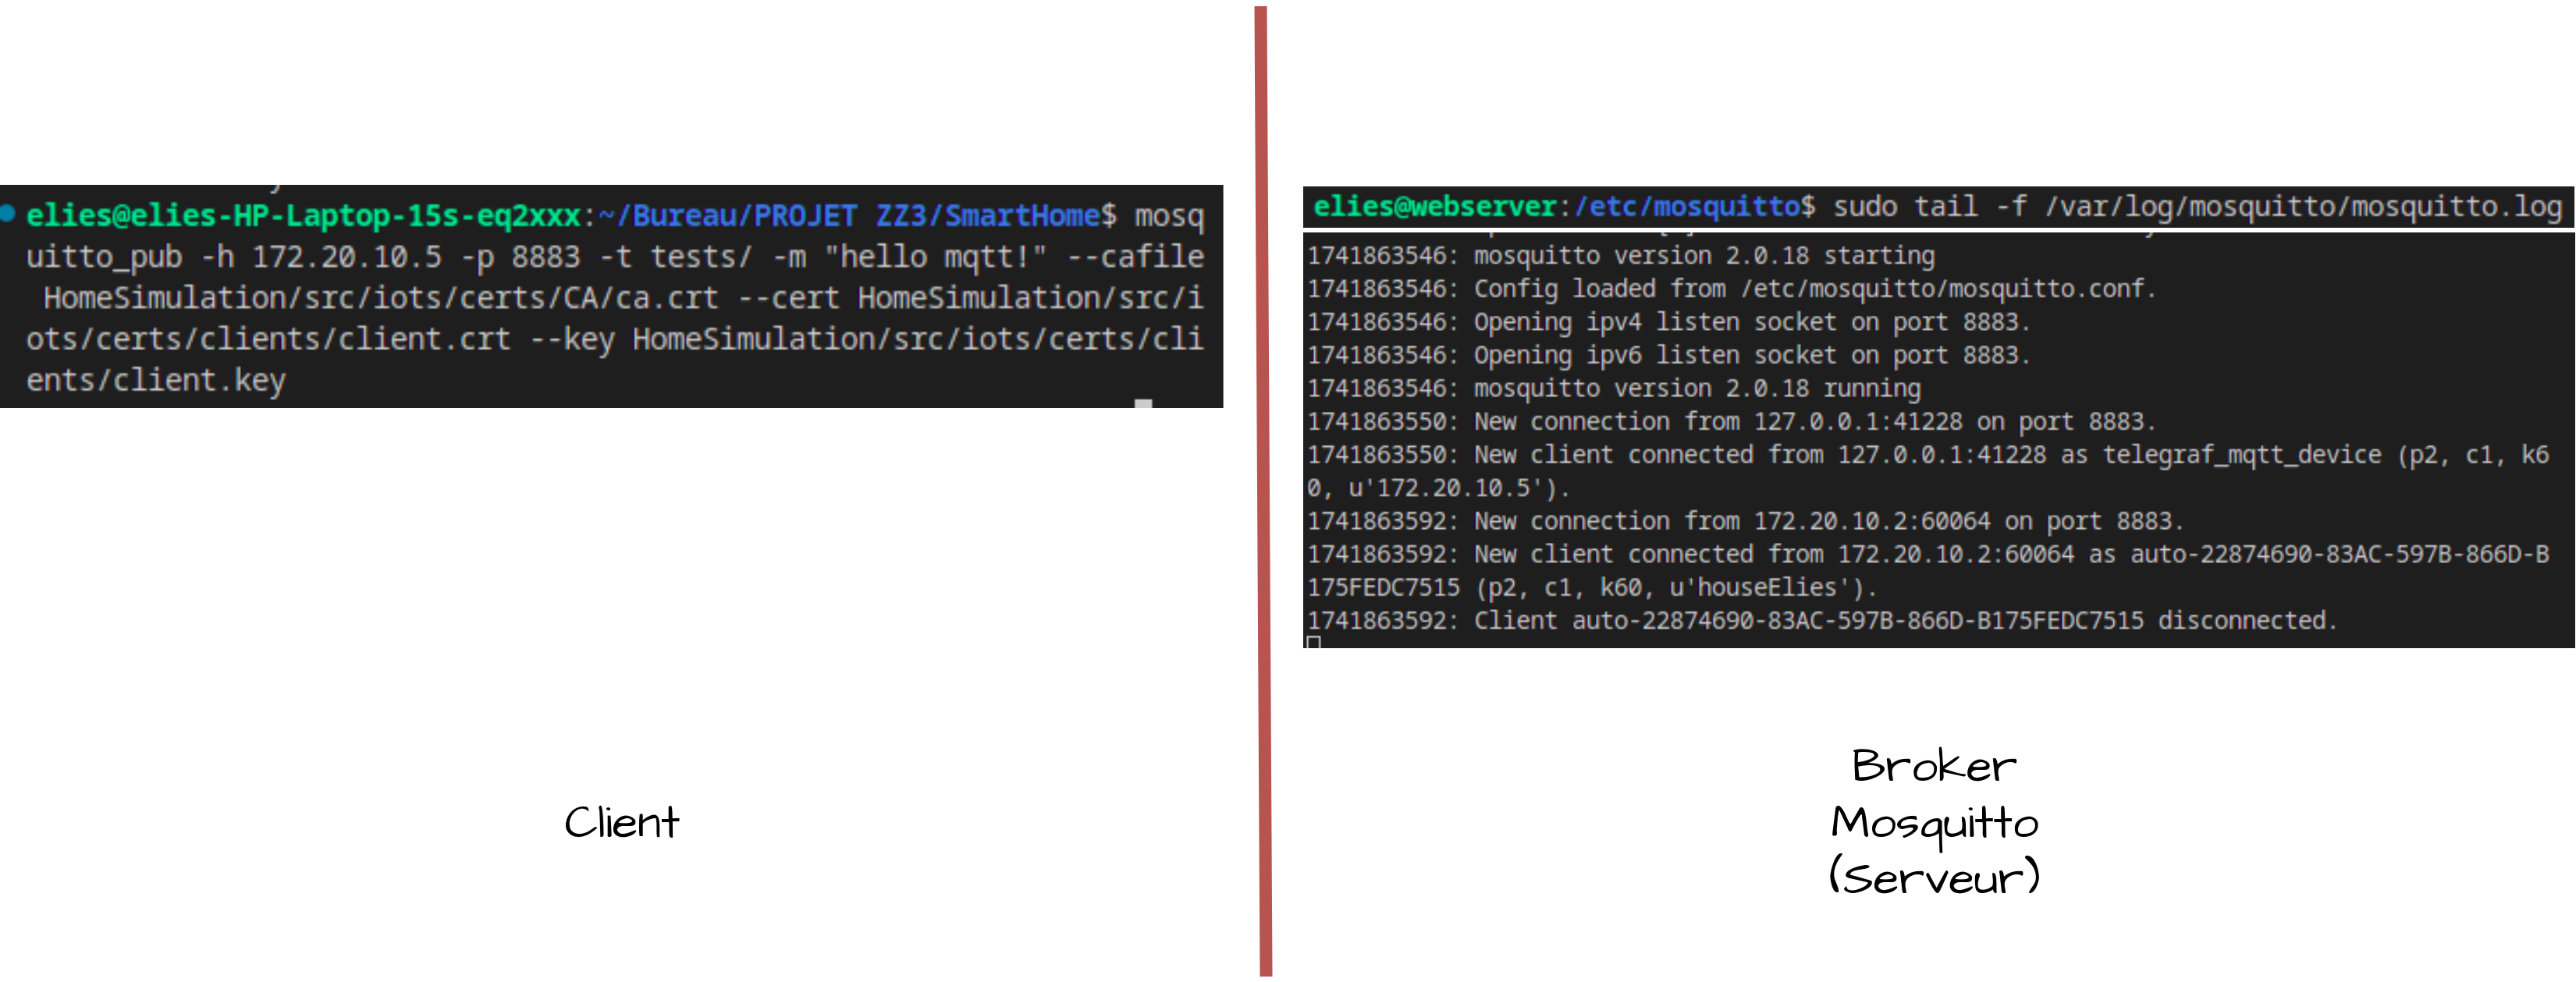
\includegraphics[width=1\textwidth]{ressources/img/preuves/emissionReceptionMosquittoValide.drawio}
		\caption{Authentification effectuée: Émission et réception effectuée avec succès}
		\label{fig:mosquittoValide}
	\end{figure}
	
	Dans la figure ci-dessus, nous pouvons nous apercevoir (par la capture d'écran du résultat du log instantané du broker) que la connexion de l'emetteur s'est correctement déroulée, et que ce client a été correctement authentifiée par le nom d'utilisateur \textbf{houseElies}. \newpage
	
	\begin{figure}[h!]
		\centering
		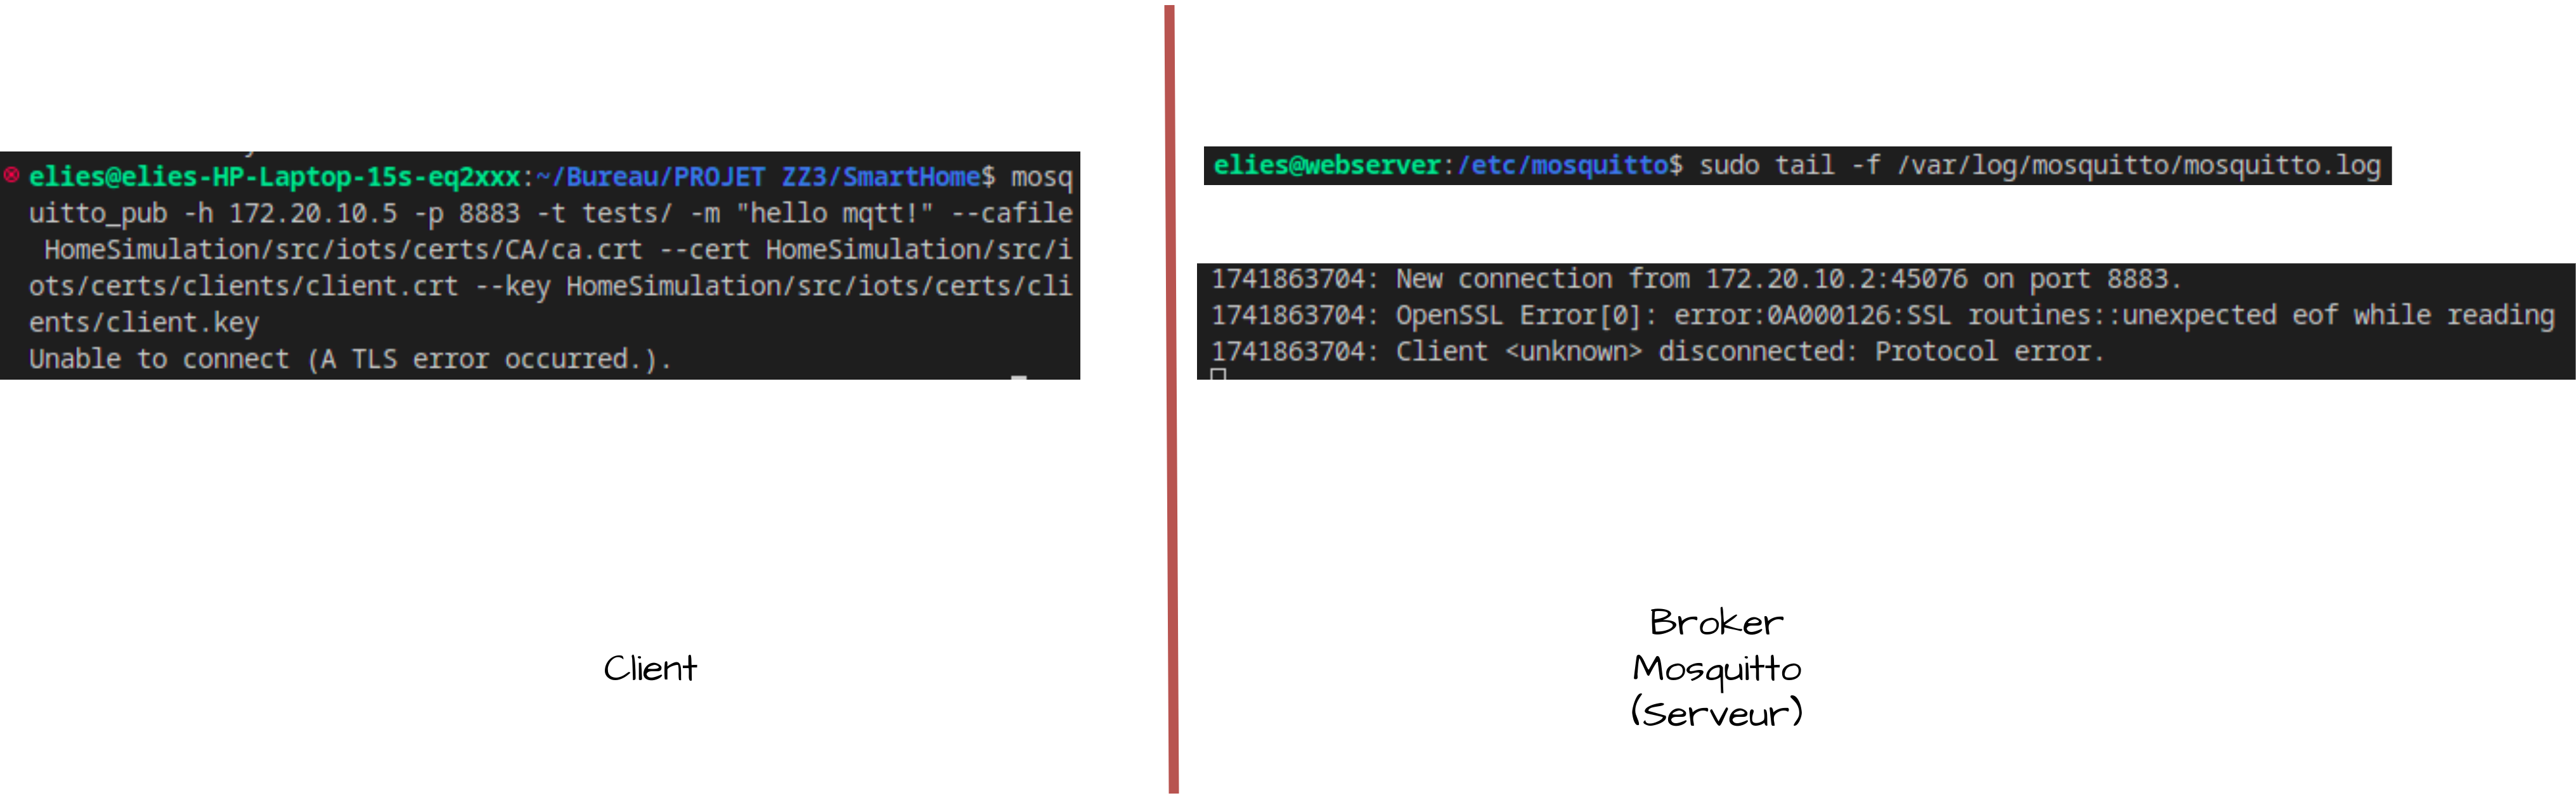
\includegraphics[width=1\textwidth]{ressources/img/preuves/emissionReceptionMosquittoInvalide.drawio}
		\caption{Authentification erronée: Émission et réception non fonctionnel}
		\label{fig:mosquittoInvalide}
	\end{figure}
	À la différence de la figure précédente, afin de prouver qu'il est nécéssaire de disposer des certificats clients valides, nous avons intentionnellement modifié la clé générée de manière à ce qu'elle soit erronée. Nous pouvons ainsi constater qu'il y a une erreur lors de la connexion de l'emmeteur et que ce dernier n'est pas parvenu à publier, ni à être identifié par le broker.
	
	
	
	\subsubsection{Intégration d'une base de données à séries temporelles}
	
	L'émission sécurisée des données depuis une adresse IP distante vers le serveur étant désormais établie, l'étape suivante consiste à assurer le stockage efficace et structuré de ces informations. L'objectif de ce projet, étant non seulement de permettre l'émission de grandes séries données en temps réel, mais aussi de pouvoir interroger et analyser des données collectées à une date ou une période spécifique. C'est pourquoi, nous avons jugé indispensable d'intégrer une base de données adaptées à des contraintes temporelles.\\
	Afin de répondre à ce problème de contraintes temporelles, nous avons utilisé une \textbf{base de donnée à séries temporelles (TSDB)}. Une base de donnée à séries temporelles est un type de base de données optimisée pour stocker et interroger des données indexées par le temps. À la différence des bases de données classiques telles que \textbf{MySQL ou PostgreSQL}, stockant les données sous forme de relation statiques, une \textbf{TSDB} permet de gérer des séries de données continues, optimisant les requêtes temporelles et sotckant de manière efficace les données horodatées.\\
	Une des plus connues est \textbf{InfluxDB}. Développée par \textbf{InfluxData}, cette base de données répond parfaitement au problème du fait qu'elle permet l'enregistrement de données évoluant dans le temps et facilite leur analyse. Contrairement à ses concurents, elle permet une écriture des donnnées rapide, ce qui est essentiel pour le temps réel. De plus, elle compresse les données de manière efficace, permettant ainsi l'optimisation de l'espace de stockage. Enfin, un des avantages clés pour notre projet, est le fait que cette base de données est capable de traiter des millions de points de données par seconde.\\
	Elle dispose de plus d'une \textbf{API Web} permettant ainsi un accès distant des données, nous verrons par la suite que cette \textbf{API} nous sera essentiels pour accèder aux données transférées.\\
	Cependant, la subtilité, est que \textbf{InfluxDB} ne supporte pas nativement le protocole \textbf{MQTT}, il est donc nécéssaire d'utiliser un composant intermédiaire afin d'assurer la transmission des messages depuis le protocole MQTT vers la base de données.\\
	Pour cela, nous avons intégré \textbf{Telegraf}, un agent de collecte de métrique concu afin d'intéragir avec différents systèmes de monitoring et bases de données.\\
	Nous avons ainsi configuré \textbf{Telegraf} pour écouter les messages publiés sur \textbf{Mosquitto} et les reformater avant des les insérer directement au sein de la base de données.\newpage
	\textbf{Telegraf} propose deux formats principaux pour insérer des données au sein d'\textbf{InfluxDB}:
	\begin{itemize}
		\item \textbf{Line Protocol:} ce format propre à \textbf{InfluxDB} optimise le sotckage ainsi que la vitesse d'écriture, il s'agit d'une syntaxe représentée sous la forme \textbf{measurement,tag=value timestamp}. Bien que très performant, ce format peut être complexe à manipuler et requière une structure rigide des données envoyées.
		
		\item \textbf{JSON:} ce format est plus lisible et universellement reconnu, facilitant le traitement et la manipulation des données. Il permet une structuration claire des informations envoyées, avec des clés explicites pour chaque valeur de mesure, ce qui facilite le débogage et l’analyse des données stockées.
	\end{itemize}
	Ainsi, pour des raisons de clarté et de lisibilité, nous avons opté pour le format \textbf{JSON}, cela nous facilitera l'écriture des algorithmes dédiés à l'envoie de données des maisons.\\
	Afin d'effectuer cela, nous avons configuré le fichier \textbf{telegraf.conf} pour utiliser le plugin \textbf{mqtt\_consumer}.\\
	Ce plugin va permettre à \textbf{Telegraf} de s'abonner à tout les \textbf{topics MQTT} qui nous permettront par la suite de récupérer les messages publiées au format \textbf{JSON}, afin d'\textbf{orchestrer automatiquement} la structuration des données au sein des tables \textbf{InfluxDB}, et de faire correspondre \textbf{les colonnes aux valeurs JSON} issues des clés correspondantes. Nous verrons plus en détail, dans la \textbf{sous-section suivante}, comment nous avons choisi de formaliser les données et ainsi structurer la base de données.\\\\
	Le schéma récapitulatif \textbf{ci-dessous} décrit le fonctionnement de \textbf{InfluxDB} et \textbf{Telegraf} au sein de l'architecture par le biais d'un exemple simple et récapitulatif des données à envoyer:
	
	\begin{figure}[h!]
		\centering
		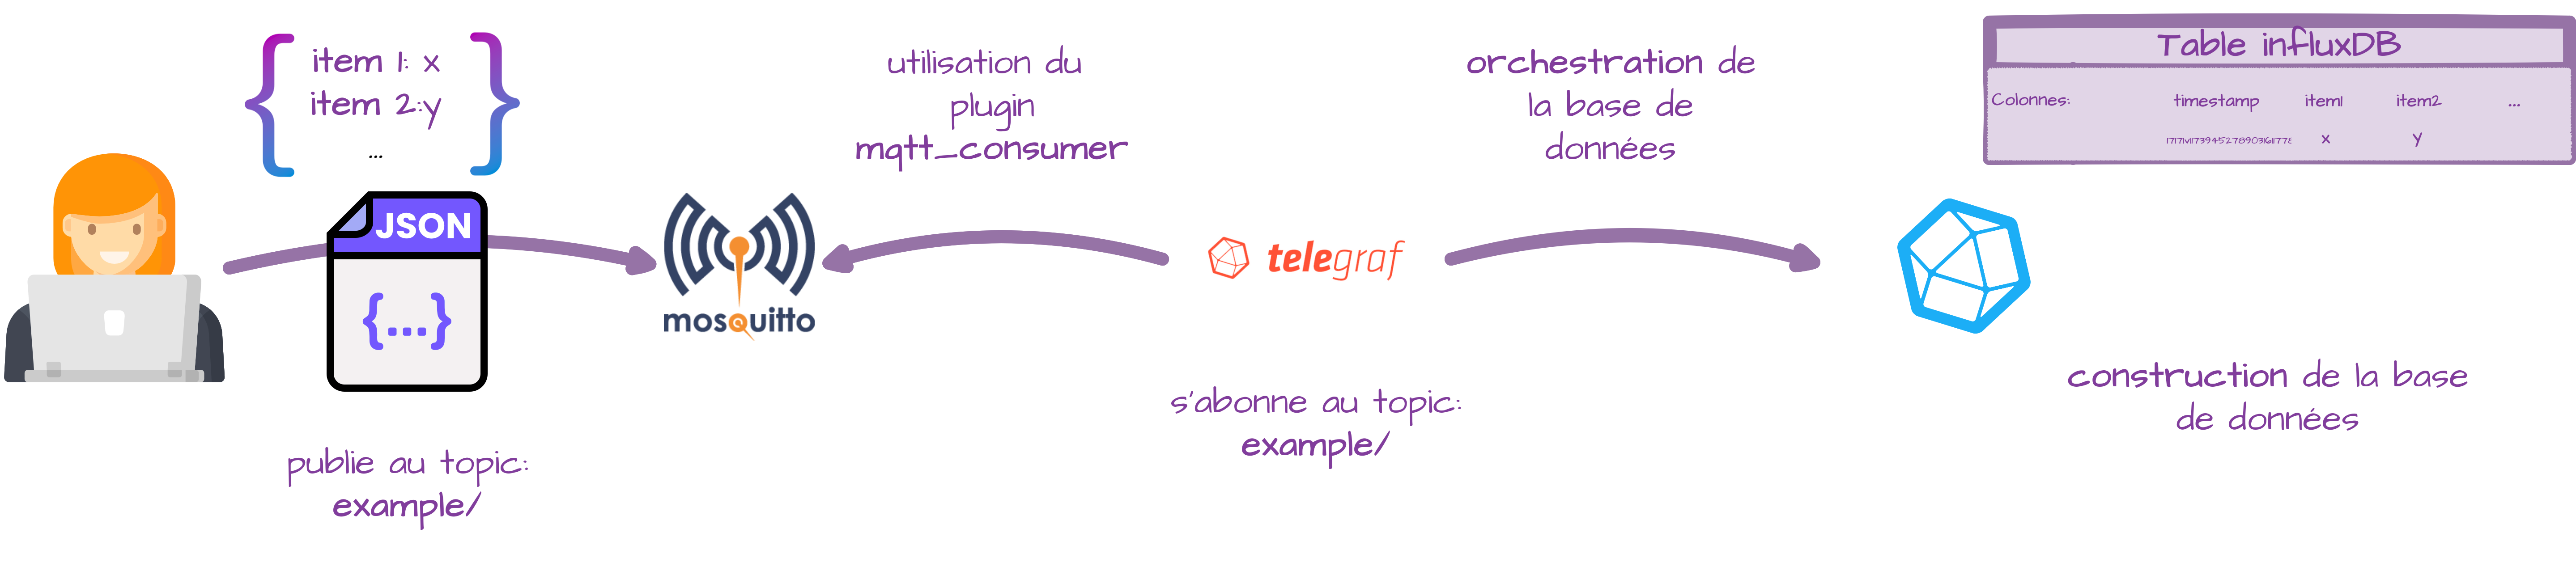
\includegraphics[width=1\textwidth]{ressources/img/shémas/archiInflux.drawio}
		\caption{Exemple de données \textbf{JSON simples} à envoyer}
		\label{fig:archiInflux}
	\end{figure}
	\vspace{1cm}
	Ainsi, l'émetteur écrit un \textbf{buffer} dans lequel il insère des données formatées en \textbf{JSON}, ces données sont envoyées à travers le protocole MQTT à un topic nommé \textbf{example/}.\\
	Ces données sont reçues au sein du broker au topic \textbf{example}, auquel s'abonne le service \textbf{telegraf} dans le but de \textbf{traduire} le format JSON recu, afin d'orchestrer et créer au sein d'\textbf{InfluxDB} la table correspondante.
	

	
	\subsection{Modélisation et Simulation d'une Maison Connectée}
	Après avoir rendu possible l'émission ainsi que le stockage de manière sécurisée et authentifiée entre un client et un serveur via le protocole \textbf{MQTTs}, nous avons entrepris la modélisation d'une maison connectée de manière réaliste.La simulation vise à reproduire les interactions d'une habitation intelligente équipée de capteurs IoT, tout en respectant les contraintes de communication définies précédemment.\\
	L'objectif de cette simulation est d'une part de permettre l'émission de séries de données depuis une maison connectée simulée, personnalisable et extensible, utilisant le protocole MQTT, et d'autre part de mettre en place un format d'envoi de données en JSON afin de permettre le remplissage de la base de données distante tout en identifiant chaque maison. 

	\subsubsection{Structuration et formalisation des données échangées}
	Dans un premier temps, avant de commencer la conception des maisons simulées, il est nécessaire de réfléchir à la structure des données au format \textbf{JSON}, que nous allons mettre en place afin de permettre une gestion efficace des données recues par les IOT's de la maison.\\
	La structuration des données repose sur une approche où chaque message transmit par la maison suit un format JSON préféfin. Le but est de garantir une compatibilité optimale avec les systèmes de stockage et de permettre ainsi un affichage correctement structuré au sein de la base de donnée.\\\\
	Afin de garantir tout cela, il nous a fallut insérer au sein de la donnée transmise divers élément permettant d'identifier la maison emettrice, mais aussi d'identifier quel IOT de la maison est concerné. Voici les clès que nous avons judicieusement choisit afin de garantir un stockage des données optimale au sein de la base de données:
	\begin{itemize}
		\item \textbf{token:} Le token est la clés primaire d'une donnée envoyée. En effet, elle permet d'identifier la maison connectée émettrice, c'est sur ce jeton que nous nous baserons afin qu'un propriétaire puisse rechercher sa maison. Nous pouvons voir le token tels que la clès de l'utilisateur, que seul lui dispose et qu'il ne doit partager personne. Nous verrons par la suite que cette clès sera généré par l'API et donnée au propriétaire lorsque ce dernier souhaitera enregistrer sa maison au sein de la base de donnée.
		
		\item \textbf{house\_name:} permet simplement de nommer la maison, il s'agit là aussi d'une clès unique, en effet elle permettera de distinguer les différents maisons au sein des sous-topics de \textbf{houses/} (explication détaillée au paragraphe suivant).
		
		\item \textbf{device\_name:} concerne l'\textbf{IOT} auquel on a capturée la donnée à envoyer (il peut s'agir d'un capteur, de l'état d'une porte d'une lumière...). Ainsi, contiendra une chaîne JSON auxquel sera stocké sont état en tant qu'information utile au propriétaire.
		
		\item \textbf{device\_location:} permet de localiser l'IOT au sein de la maison, cette information pourra être utile dans le cas où l'on souhaiterait établir une cartographie de la maison au sein de l'interface graphique, et que le propriétaire puisse ainsi avoir une vue globale de sa propriété, avec l'ensemble des capteurs présent à leur localisation spécifiques.
		
		\item \textbf{type:} Cette clés permettra d'organiser chaque \textbf{IOT} en fonction de leur rôle attribué (capteur\_lumière...), cela pourra ainsi permettre d'ajouter un filtre en plus dans le cas où on suppose qu'un propriètaire veuille récupérer les données issues de l'ensemble des lampes de sa maison par exemple.
		
		\item \textbf{values:} Cette clés pourra stocker un tableaux contenant une ou plusieurs donnée, correspondant à l'état d'un \textbf{IOT} à un instant donné.
	\end{itemize}
	
	Ainsi, chaque série de données envoyées par la maison est constituée d'une ou plusieurs données au format JSON composées des clés spécifiés.\\
	Voici un exemple de donnée envoyé par une maison à un un instant donné composé uniquement d'un capteur de lumière:
	
	\begin{lstlisting}
	{
		"house_name": "eliesHouse",
		"house_token": "Wdp4HCPNvC3wHnvSfSwmVknhLuHtjUkoIzG6zPno",
		"device_name": "lamp_kit",
		"device_id": 1,
		"device_location": "kitchen",
		"type": "light_sensor",
		"values": { "state": 0 }
	}
	\end{lstlisting}
	
	\paragraph{Disposition des Topics}
	
Un autre élément permettant la structuration des données émises par les maisons ainsi que l'organisation de ces dernières est la disposition des topics.
En effet, il est important de distinguer les différents \textbf{sous-topics} du topic racine \textbf{houses}, contenant l'ensemble des maisons, qui elles-mêmes incluent dans des sous-topics les différents types d'IoT.

L'organisation des \textbf{topics} suit la hiérarchie suivante :
\begin{itemize}
	\item \textbf{houses/} : Racine des topics, regroupant toutes les maisons connectées.
	\item \textbf{houses/<house\_name>/} : Chaque maison possède un sous-topic dédié identifié par son nom unique.
	\item \textbf{houses/<house\_name>/<device\_type>/} : Le but est de garantir une catégorisation des équipements par type (ex: TYPE\_LIGHT, TYPE\_HUMIDITY...).
	\item \textbf{houses/<house\_name>/<device\_type>/<device\_name>} : Le dernier niveau représente un équipement précis (par exemple lampe, capteur de température).
\end{itemize}
	\vspace{1cm}
	Voici un exemple de topics auquel l'information de l'état de la lampe de la maison est publié:
	\textbf{houses/eliesHouse/TYPE\_LIGHT/lamp\_kit}\\
	

	Cette organisation permet une classification logique et structurée des messages publiés, facilitant ainsi la récupération et le traitement des données par les abonnés spécifiques aux topics concernés.\\
	
	Afin de garantir cette organisation, nous avons configuré avant de passer à la création du simulateur configure telegraf. Le plugin \textbf{mqtt\_consumer} permet de hierarchiser les topics auxquels seront envoyées les donénes et d'établir des strutures précises.
	\subsubsection{Conception de l'architecture logicielle de la simulation}
	La conception de l'architecture logicielle de la simulation repose sur une structure modulaire extensible et permettant d'intégrer plusieurs maisons connectées, entièrement personnalisable, pouvant contenir un très grand nombre d'appareils \textbf{IOTs}. Nous avons choisit de développer cette architecture en Python en raison de sa flexibilité et du fait qu'il contient des bibliothèques permettant l'implémentation des communication réseau via le protocole MQTT de manière simple et rapide.\\
	
	Chaque maison connectée est modélisée sous forme d'une classe Python encapsulant l'ensemble des capteurs et des dispositifs présents dans l'habitation.Ces équipements sont eux-mêmes représentés par des classes spécifiques dérivées d'une classe abstraite \textbf{Device}, permettant d'uniformiser la gestion des données et des envois MQTT.\\
	
	\paragraph{Principales composantes de l'architecture logicielle}
		Voici les fonctionnalités que nous avons implémenté au sein de l'architecture logiciel:

	\begin{itemize}
		\item \textbf{House} : Classe représentant une \textbf{maison connectée}. Chaque instance est associée à un token unique et gère un ensemble d'équipements IoT.
		\item \textbf{Device} : Classe abstraite représentant un dispositif connecté (capteurs, actionneurs). Les classes spécifiques (ex: \textbf{LightSensor}, \textbf{HumiditySensor}) en héritent.
		\item \textbf{Main}: Cette classe agit comme un point central au sein de cette simulation, en effet, elle initialise les maisons connectée ainsi que leur capteurs, elle orchestre l'émission des données en fonction d'un intervalle défini et elle établit et maintient la connexion \textbf{MQTT} pour chaque maison. 
	\end{itemize}
	
	\begin{figure}[h!]
		\centering
		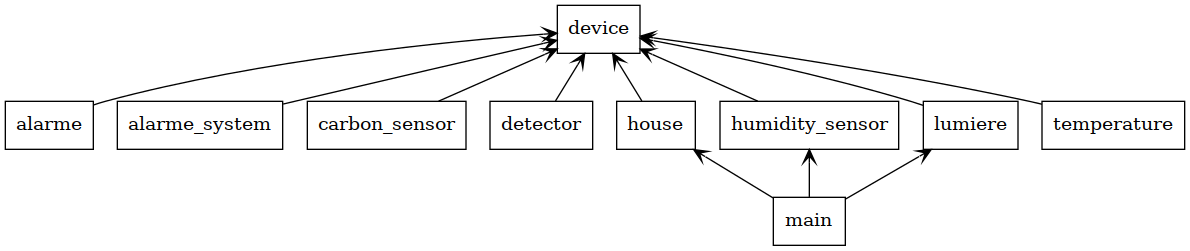
\includegraphics[width=1\textwidth]{ressources/img/shémas/housesimulationDiagram}
		\caption{Architecture logicielle proposée de notre simulateur de maisons connectées}
		\label{fig:archiMaisonConnectées}
	\end{figure}
	
	\paragraph{Envoies des données JSON à chaque classe IoT}

	\paragraph{Implémentation du Protocole MQTT} Afin d'implémenter le protocole \textbf{MQTT} nous avons utilisé la bibliothèque \textbf{paho-mqtt}, qui est une implémentation légère du protocole en Python. Cette bibliotèque permet la gestion complète des communications entre les clients \textbf{MQTT} et le \textbf{broker}, en facilitant la publication ainsi que la souscription aux topics définis.\\
	Nous avons dans un premier temps vérifié le fonctionnement de manière non sécurisé (sans SSL/TLS), afin de vérifier si l'émission des données au format conçu fonctionnait tels que prévu, avant d'ajouter les \textbf{certificats SSL/TLS} afin de permettre l'implémentation du protocole MQTTs. 

	
	\paragraph{Implémentation du protocole MQTTs} La bibliothèque \textbf{paho-mqtt} que nous avons utilisée supporte l'intégration de certificats \textbf{SSL/TLS}. Afin d'intégrer ces certificats, la bibliothèque dispose de l'objet \textbf{mqtt.Client()} contenant une méthode \textbf{tls\_set(ca\_certs, certfile, keyfile)}. Cette méthode prend en paramètre le chemin du certificat de l'autorité de certification, du propriétaire ainsi que la clé privée de ce dernier.\\
	En appelant ensuite la méthode \textbf{publish()} de la classe \textbf{mqtt.Client}, il nous sera possible d'envoyer les données en utilisant ces certificats et ainsi garantir une authentification sécurisée.
	
	Cette implémentation garantit une transmission fiable et sécurisée des données IoT simulées, tout en respectant les bonnes pratiques d’authentification et de chiffrement des communications réseau.
	
	\paragraph{Diagramme UML décrivant l'architecture des classes du simulateur} Afin de résumer l'architecture des classes du simulateur, voici le diagramme UML:

		\begin{figure}[h!]
		\centering
		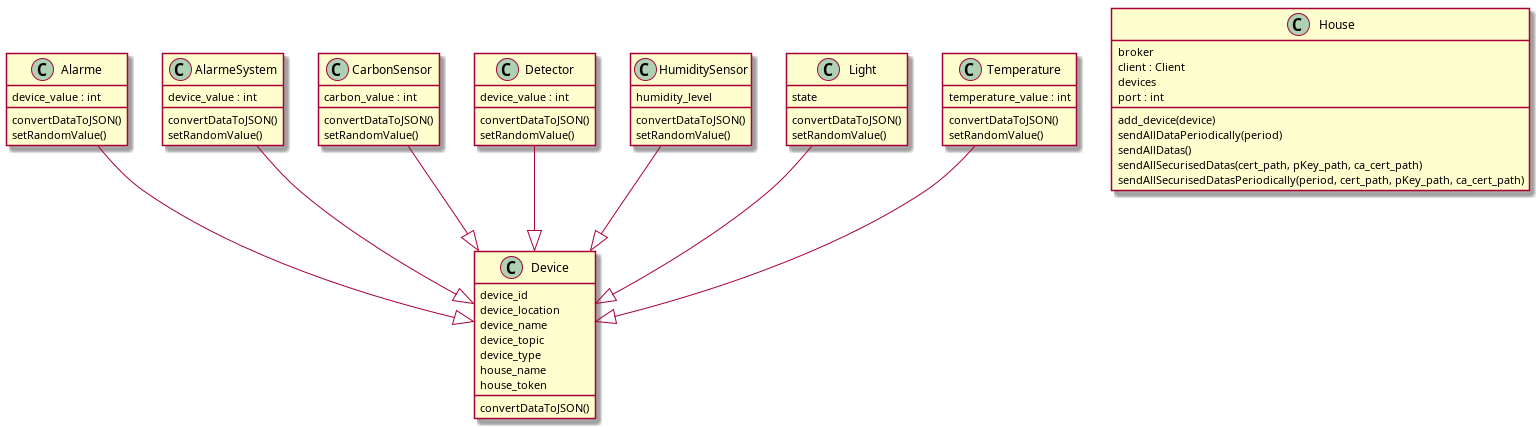
\includegraphics[width=1\textwidth]{ressources/img/shémas/housesimulationUML}
		\caption{Diagramme UML du \textbf{simulateur de maisons connectées}}
		\label{fig:umlMaisonConnectées}
		\end{figure}
	
	\section{Mise en place d'une API Web}
	Afin d'automatiser \textbf{l'authentification des utilisateurs}, d'\textbf{accéder aux données} et de permettre par la suite la \textbf{possibilité de création d'applications multiplateformes}, nous avons mis au point une \textbf{API Rest}.\
	Cette \textbf{API Rest} est l'élément principal de l'architecture. En effet, elle constitue le cœur de l’application, jouant un rôle central dans la gestion des données acquises issues des maisons connectée. Elle permet notamment :

	\begin{itemize}
		\item L’\textbf{authentification} et l’\textbf{identification} des maisons connectées.
		\item L’automatisation de la \textbf{gestion des certificats SSL/TLS} afin de garantir l'authentification des maisons connectées, et de la fiabilité des données envoyées par ces dernières.
		\item L’exposition d’une interface permettant aux applications clientes (bureau, mobile, web...) d’interagir avec le système.
	\end{itemize} 

	\subsection{Architecture logicielle de l'API et choix technologiques}
	
	Afin de mettre en place l'\textbf{API Rest}, que nous avons nommé \textbf{SmartHome API}, nous avons choisis d'utiliser le framework \textbf{Laravel} et d'ainsi développer l'application en PHP.
	
	\subsubsection{Choix du framework Laravel}
	\textbf{Laravel} est un frameworl PHP moderne et puissant, basé sur une architecture \textbf{MVC}, permettant de structurer et d'organiser de manière efficace le développement d'applications web.\\
	Dans le cadre de notre projet, l'utilisation de ce framework présente de nombreux avantages, notamment en matière de \textbf{sécurité} et de \textbf{gestion des bases de données}.\\
	Les fonctionnalitées clés de Laravel qui nous ont convaincus à l'utiliser afin de développer l'API sont:
	\begin{itemize}
		\item \textbf{La sécurité avancée}: Laravel propose nativement une protection contre les attaques courantes tels que les \textbf{injection SQL}, les \textbf{failles XSS} et les attaques \textbf{CSRF}, qui consistent à falsifier les reqûetes intersites.
		
		\item \textbf{ORM Eloquent}: Un système de gestion de base de donnée en optimisé permettant de manipuler des données en utilisant des notions simple de Partie orientée objets, plutôt qu'avec des requêtes SQL classiques. Il permet d'effectuer des opérations \textbf{CRUD} sur la base de données.
		
		\item \textbf{Migrations de bases de données}: Laravel permet de gérer la structure des base de données par le biais d'un système de versionnement. L'objectif est de faciliter la création, la mise à jour ainsi que la synchronisation des bases de données entre les environnements de développement et de production.
		
		\item \textbf{Gestion des routes et des contrôleurs}: Laravel offre un système de routage facile à comprendre, permettant d'associer de manière simple les requêtes aux méthodes des contrôleurs
	\end{itemize}
	En plus des fonctionnalités citées, \textbf{Laravel} dispose d'une communauté importante ainsi que d'une documentation très complète, nous ayant permit d'effectuer ce projet pour le mieux.
	
	\subsubsection{Déploiement de Laravel au sein du serveur Virtuel}
	Afin de pouvoir développer l'API, nous avons dans un premier temps déployé le Framework \textbf{Laravel}, au sein de notre serveur virtuel.\\
	Ce processus de déploiement s'est déroulé en plusieurs étapes.
	\paragraph{Installation des dépendances requises}
	Avant d'installer \textbf{Laravel}, nous avons dans une première partie fait en sorte de rendre l'environnement de notre serveur, compatibles avec ses exigences.\\\\
	Nous avons tout d'abord installer \textbf{PHP7.4}, qui est le language supporté par Laravel. Nous avons choisis cette version du fait qu'lle est largement compatible avec \textbf{Laravel}, et bénéfice encore de mises à jour de sécurité. \\ 
	Ensuite, nous avons installé \textbf{pdo}, une interface qui permet d'interagor avec les bases de données SQL tels que \textbf{MySQL}, qui est par ailleurs la base de donnée que nous avons utilisés afin de stocker les informations relatifs à l'identification des maisons au sein de l'\textbf{API} et d'\textbf{InfluxDB}.\\
	Nous avons installé \textbf{Apache2}, un serveur web qui nous permettera d'éxécuter Laravel, en raison de sa compatibilité native avec PHP, et de sa facilité de configuration. \\
	Enfin, afin de faciliter l'installation ainsi que les mises à jour des packages \textbf{Laravel}, nous avons installer \textbf{Composer}, un gestionnaire de dépendance PHP, couramment utilisé en complément de \textbf{Laravel}.\\\\
	Après avoir installés ces dépendances, nous avons installer \textbf{Laravel} et mit au point le projet constituant l'API, que nous avons appelé \textbf{SmartHomeAPI}.
	

	
	\paragraph{Configuration de SmartHomeAPI}
	La configuration de l'\textbf{API} représente une étape fondamental à son fonctionnement. En effet, elle permet de définir quels services nous allons utilisé, quels ports nous allons. choisir...\\
	Afin de faire cela, nous avons configuré le fichier \textbf{.env}, un fichier caché de \textbf{Laravel} permettant la configuration ainsi que la dzfinition des variables d'environnements spécifiques à l'application. Il permet de spécifier les paramètres d'accès à la base de données, le nom de l'application...\\
	Voici un des extraits de notre fichier de configuration \textbf{.env}, contenant les informations permettant de lier chaque services essentiels au projet à son port d'utilisation au sein du serveur:
	
	\begin{lstlisting}
		# On specifie les informations principales directement liée à l'API ainsi qu'à son accessibilité
		APP_NAME=SmartHomeAPI
		APP_ENV=local
		APP_KEY=base64:mrAfKToAj/ycaELKT04bx4Zl9Lq/5de3EQ2xTK5LWak=
		APP_DEBUG=true
		APP_TIMEZONE=UTC
		APP_URL=http://172.20.10.2:8000
		...
		# On spécifie l'utilisation de mySql et des informations relatives au sein du serveur
		DB_CONNECTION=mysql
		DB_HOST=127.0.0.1
		DB_PORT=3306
		DB_DATABASE=intelighouseDB
		DB_USERNAME=elies
		DB_PASSWORD=admin
	\end{lstlisting}
	\paragraph{Configuration d'Apache2}
	\textbf{Apache2} est un serveur web open-source, que nous avons utiliser afin d'héberger notre API.\\
	Il permet de traiter des requêtes HTTP et de servir les différentes pages aux clients connectés.\\
	Ainsi, \textbf{Apache 2} va assurer la communication entre l'hutilisateur souhaitant avoir accès aux données de sa maison et le serveur virtuelle.\\
	La configuration d'Apache2 est essentielle à la mise en place de notre projet \textbf{Laravel}, afin de permettre un accès sécurisé et contrôlé à l'API.\\\\
	Dans un premier temps, nous avons mit en place un \textbf{VirtualHost}, une directive de configuration d’Apache2 qui permet d’héberger plusieurs sites web ou applications au sein d'un même serveur, en définissant des règles spécifiques à chaque hôte.Dans notre cas, nous avons créé un fichier de configuration dédié nommé \texttt{intelighouse.conf} afin d’exposer notre API SmartHome sur un port spécifique que nous avons attribué: \textbf{Le port 8000}.\\
	Le fichier de configuration \textbf{intelighouse.conf} a été créé au sein du répertoire \texttt{/etc/apache2/sites-available/} avec le contenu suivant :
	
	\begin{lstlisting}
	<VirtualHost *:8000>
		ServerName 172.20.10.5
		DocumentRoot /var/www/SmartHomeAPI/SmartHomeApi/public
		
		<Directory /var/www/SmartHomeAPI/SmartHomeApi/public>
		AllowOverride All
		Require all granted
		</Directory>
	</VirtualHost>
	\end{lstlisting}
	
	La configuration ci-dessus, spécifie ainsi que l'application \textbf{Laravel} écoutera sur le \textbf{port 8000}, et que le \textbf{VirtualHost} sera associée à l'adresse IP \textbf{172.20.10.5}. Ainsi, l'API sera accessible via l'url: \textbf{http://172.20.10.5:8000/}, depuis le client.\\
	Enfin, on associe le \textbf{VirtualHost} au répértoire dans lequel se situe l'application Larave, et attribuons à appache2 les droits nécéssaires afin d'activer les fichiers \textbf{.htaccess} et d'y définir des règles.
	
	\paragraph{Configuration de la base de données}
	Nous avons aussi à ce moment là mit en place la base de données contenant les \textbf{intelighouseDB}, dans laquelle nous avons généré depuis \textbf{Laravel}, les migrations permettant la création de la table \textbf{houses} qui stockera les maison, identifié par un nom de \textbf{maison}, un \textbf{mots de passe} ainsi qu'un \textbf{token}.
	
	\begin{figure}[h!]
		\centering
		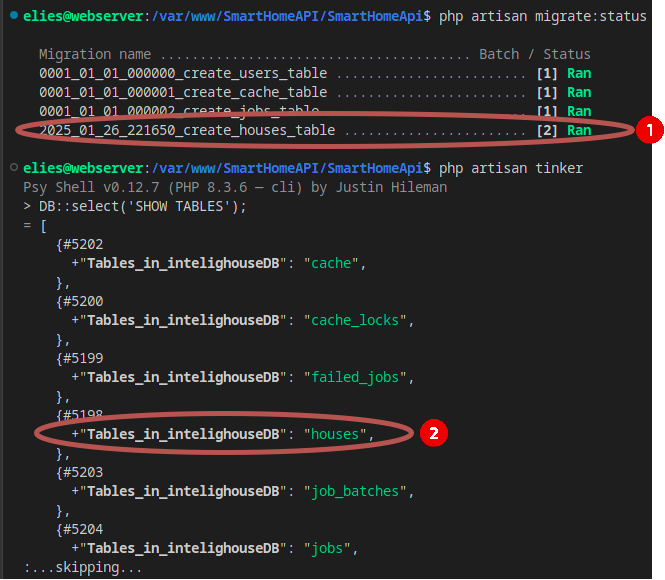
\includegraphics[width=0.5\textwidth]{ressources/img/preuves/preuveMigration}
		\caption{Vérication de la création de la \textbf{base de données}}
		\label{fig:preuveBDD}
	\end{figure}
	\newpage
	On constate ainsi en analysant l'image ci-dessus deux points:
	\begin{itemize}
		\item La commande \textbf{php artisan migrate.status} permet de ici de vérifier le statut quand aux migrations déployées au sein du projet, nous pouvons voir que la migration \textbf{create\_house\_table} a bien été crée. 
		\item La commande \textbf{DB::seect('SHOW TABLES')} permet de vérifier quels tables sont contenues en base, ce qui nous permet ainsi de constater que la table \textbf{houses} issues de la migration \textbf{create\_houses\_tables} a bien été crée au sein de \textbf{intelighouseDB}.
	\end{itemize}
	
	\subsubsection{Architecture de l'API}
	SmartHomeAPI repose sur une architecture suivant l'architecture MVC définit par le framework \textbf{Laravel}, faisant ainsi d'elle une architecture modulaire et extensible.\\
	L'architecture permet de gérer les maisons connectés de leur authentication, ainsi que la récéption des données issues des maisons authentifié.\\
	L'API suit le modèle \textbf{RESTful}, permettant ainsi une séparation claire des résponsabilités ainsi qu'une compatibilité avec divers applications clientes (\textit{cf.} section 3.3 \textbf{Surveillance des données avec une interface graphique}).
	
	\paragraph{Structure globale de l'API}
	
	L'API est structurée en plusieurs composants:
	\begin{itemize}
		\item \textbf{Les routes}: Elles permettent de définir les \textbf{points d'entrée} de l'API, c'est à dire les différents URL par lesquelles les clients vont effectuer leurs requêtes de manière à accéder au service voulu. Ces points d'entrées ont étaient mis en place au sein du fichier \texttt{routes/api.php}.
		\item \textbf{Les contrôleurs}: Ils permettent d'acheminer les commandes des modèles. Au sein de l'\textbf{API}, deux contrôleurs sont centraux: Il y a tout d'abord \textbf{HouseController}, qui permet de gérer la création de maison, l'authentification, et il y a \textbf{InfluxDBController}, qui permet de gérer la récupération des données des divers maisons, authentifié par token, via l'API \textbf{InfluxDB} interne au serveur.
		\item \textbf{Le Modèle}: Le modèle dans notre cas contient la représentation spécifiques des données spécifiques d'une maison stockée au sein de la base de données \textbf{MySQL}.
		\item \textbf{Base de données} L'API accès à deux bases de données au sein du serveur virtuelle: La base de donnée liée au séries de donnée de chaque maison, aucuel l'accès se fait par le biais de l'API \textbf{InfluxDB}, ainsi que la base de données MySQL contenant les utilisateurs. Les deux base de données correspondent leurs information par le biais d'une clès appelée \textbf{token}, généré lorsque l'utilisateur effectue une requête de création de maison à \textbf{SmartHomeAPI}.
	\end{itemize}
	
	\paragraph{Structure des bases de données} La figure ci-dessous décrit la structure de la table \textbf{House} associée à sa table \textbf{intelighouse}, situées au sein de bases de données de type différents.
		\begin{figure}[h!]
			\centering
			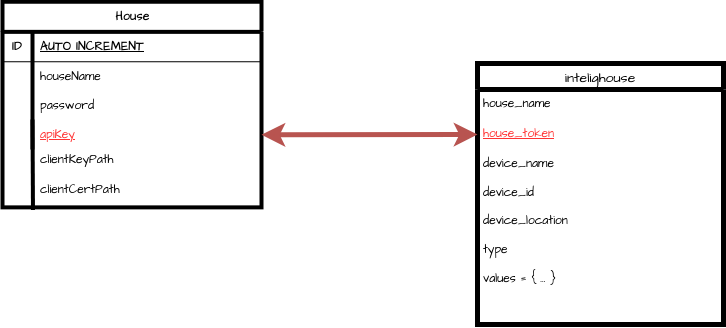
\includegraphics[width=0.5\textwidth]{ressources/img/shémas/BDDS_Archi}
			\caption{Association d'une Table Maison de Smarthouse à ses séries de données temporelles collectées}
		\label{fig:archBDDs}
		\end{figure}
		
		La table \textbf{House}, situé au sein de la base de donnée \textbf{MySQL}, structurée à partie du modèle \textbf{House.php}, contient les informations liées à l'authentification d'une \textbf{maison connectée} au sein de l'architecture globale du serveur:
		\begin{itemize}
			\item \textbf{item} est identifiant unique s'auto-incrémentant au sein de la base à chaque création de maison de la part d'utilisateur.
			\item \textbf{houseName} est nom unique de maisons au sein de la base de données relationnel.
			\item \textbf{password} est le mots de passe haché en \textbf{bcrypt} du propriétaire de la maison, lors de son authentification.
			\item \textbf{apiKey} est une clé API unique généré par l'API, elle permet d'identifier les maison au sein des deux bases de données. 
			\item \textbf{clientKeyPath} et \textbf{clientCertPath} constituent les chemins des certificats client au sein du serveur.
		\end{itemize}
		Les valeurs de la tables \textbf{intelighouse} ont été décrites à la fin de la partie \textbf{Structuration et formalisation des données échangées}, la seul spécificité est le fait que \textbf{house\_token} constitue une forme de \textbf{clé étrangére} liée à la valeur de \textbf{apiKey} situé au sein de la base de données \textbf{MySQL}.
		
	\paragraph{Fonctionnement des routes}
	La spécification des routes est contenue au sein du fichier \texttt{routes/api.php}. Ce fichier contient un \textbf{groupe de routes} préfixé \textbf{house}, permettant la mise en œuvre des action à réaliser par l'api en fonction des requêtes émises par l'utilisateur.\\
	Au sein de notre API, cinq routes ont étés mise en œuvre permettant le fonctionnement voulu de l'\textbf{API} conforme aux besoins nécessaire à l'architecture.
	
	

\begin{table}[h]
	\centering
	\small % Réduit la taille de la police pour éviter les débordements
	\renewcommand{\arraystretch}{1.2} % Augmente l'espacement des lignes pour une meilleure lisibilité
	\begin{tabularx}{\textwidth}{|X|c|X|X|}
		\hline
		\textbf{Route} & \textbf{Méthode} & \textbf{Fonction associée} & \textbf{Description} \\
		\hline
		\texttt{/api/house/create} & POST & \textbf{HouseController@create()} & Création d’une maison avec génération des certificats SSL et d’une clé API en retour JSON \\
		\hline
		\texttt{/api/house/data} & GET & \textbf{InfluxDBController@
		getAllData()} & Récupération de toutes les données associées à une maison \\
		\hline
		\texttt{/api/house/latestData} & GET & \textbf{InfluxDBController@
			getLatestData()} & Récupération des dernières données enregistrées \\
		\hline
		\texttt{/api/house/dataBySensor} & GET & \textbf{InfluxDBController@
			getDataBySensor()} & Récupération des données pour un type de capteur spécifique \\
		\hline
		\texttt{/api/house/dataAverage} & GET & \textbf{InfluxDBController@
			getAveragebySensor()} & Moyenne des données d’un capteur sur une période donnée \\
		\hline
	\end{tabularx}
	\caption{Routes de l'API et leurs descriptions}
	\label{tab:api_routes}
\end{table}
	
	\paragraph{Résumé de l'architecture}L'API suit une architecture MVC et permet l’authentification sécurisée des maisons ainsi que la récupération de leurs données en temps réel. Lorsqu’un propriétaire enregistre sa maison, l’API génère un token unique et des certificats SSL, stockant les informations dans une base MySQL. Pour accéder aux données IoT, le client envoie des requêtes à l’InfluxDBController, qui interroge InfluxDB via une API dédiée et retourne les mesures correspondant au token. Cette architecture garantit une gestion efficace des maisons connectées et de leur données, ainsi qu'une automatisation du placement des certificats, et clés privé au sein du dossier \textbf{cert} du simulateur.\\
	
	\begin{figure}[h!]
		\centering
		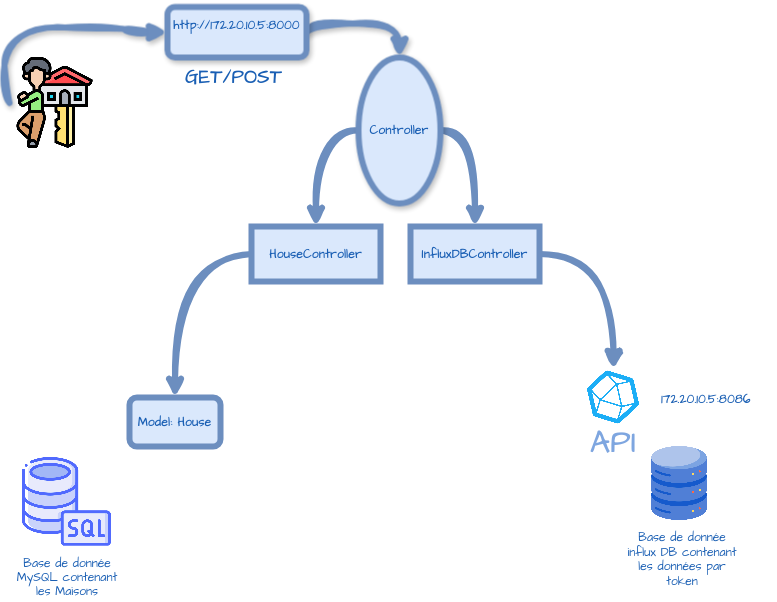
\includegraphics[width=0.75\textwidth]{ressources/img/shémas/archiAPI}
		\caption{Architecture de SmartHomeAPI}
		\label{fig:archAPI}
	\end{figure}
	
	
	\subsection{Tests de l'API avec Postman}
	
	Dans cette sous-section, nous allons tester l’\textbf{API REST} à l’aide de \textbf{Postman}, un outil permettant d’envoyer \textbf{des requêtes HTTP} et d’\textbf{analyser les réponses du serveur}. \textbf{Postman} facilite le développement, le test et la validation des API en simulant des appels client sans nécessiter d’interface graphique spécifique. Il nous a été particulièrement utile lors du développement de l'API.
	
	Le tests de l'API est constitué de 3 phases :
	\begin{itemize}
		\item \textbf{Créer un propriétaire} et associer son token à la maison connectée simulée, et \textbf{récupérer les certificats} nécessaires à l’authentification auprès du broker MQTT.
		\item \textbf{Simuler} l’envoi de données depuis la maison connectée.
		\item \textbf{Vérifier} que l’API accède correctement aux données stockées dans InfluxDB.
	\end{itemize}
	
	

	
	\paragraph{Création d'un Propriétaire} La première requête consiste à associer un propriétaire à une maison connectée. Pour ce faire, il enregistre sa maison au sein de la base de données du serveur via l’API REST. En réponse, l’\textbf{API} retourne plusieurs éléments \textbf{essentiels à l’identification et à la sécurisation des échanges} :
	
	\begin{itemize}
		\item \textbf{Le Token:} Un identifiant unique attribué à la maison. Il agit comme une clé d’authentification, connue uniquement du propriétaire et stockée dans la maison connectée. Ce token est utilisé pour accéder aux données des capteurs et garantir que seul le propriétaire peut consulter l’état de son domicile.
		
		\item \textbf{Le certificat d’autorité (CA.crt):} Nécessaire pour toute communication sécurisée avec le \textbf{broker MQTT}, ce certificat permet de \textbf{vérifier l’authenticité du serveur et d’établir une connexion sécurisée}
		
		\item \textbf{clientKey:} Il s’agit de la clé privée propre à la maison connectée, générée lors de son enregistrement. Elle est essentielle pour établir une connexion sécurisée et authentifiée avec le \textbf{broker MQTT}, garantissant que \textbf{seule cette maison spécifique est autorisée à publier des messages}.
		
		\item \textbf{cientCrt: }Ce certificat est associé \textbf{à la clé privée} et permet d’\textbf{authentifier la maison auprès du broker MQTT}. Il assure que seules les maisons disposant d’un certificat valide pourront être reconnues et communiquer avec le serveur, empêchant ainsi \textbf{toute tentative d’usurpation d’identité}. 
	\end{itemize}
	
	\begin{figure}[h!]
		\centering
		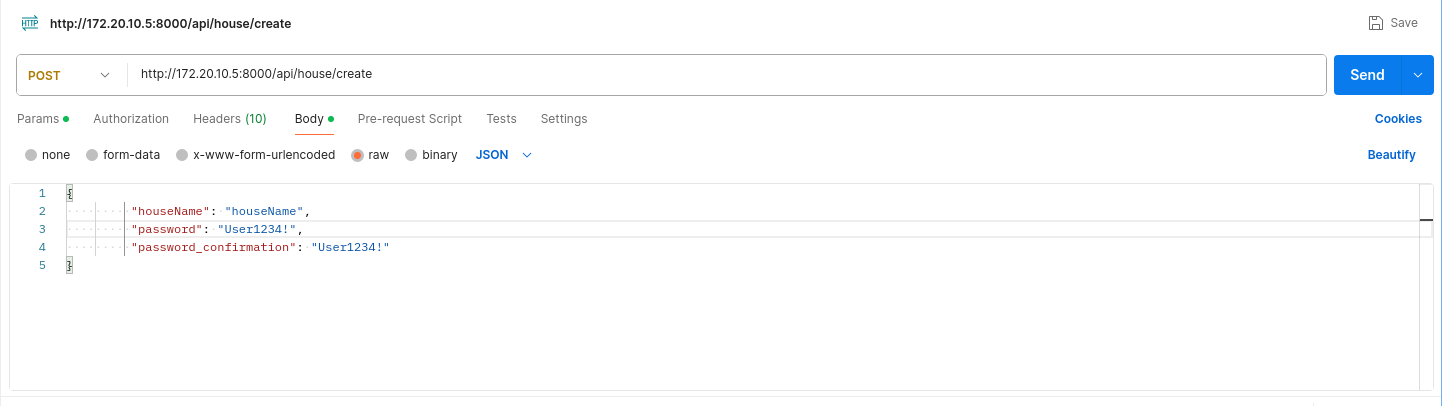
\includegraphics[width=0.75\textwidth]{ressources/img/preuves/creerMaisonRequete}
		\caption{Requête d'enregistrement d'un propriétaire associable à sa maison}
		\label{fig:preuveRequeteCreate}
	\end{figure}
	
	\begin{figure}[h!]
		\centering
		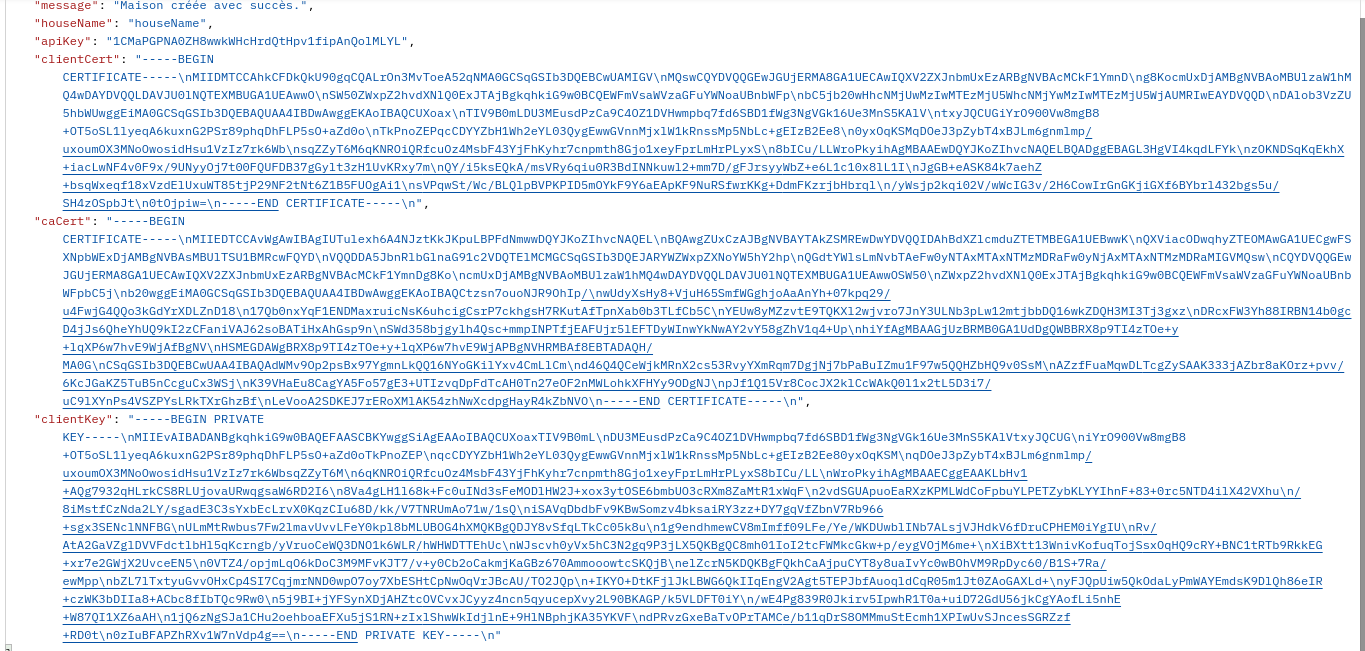
\includegraphics[width=0.75\textwidth]{ressources/img/preuves/creerMaisonReponse}
		\caption{Réponse de \textbf{SmartHomeAPI} après enregistrement réussis}
		\label{fig:preuveResponseCreate}
	\end{figure}
	
	\paragraph{Association d'un propriétaire à sa maison et envoie des données}
		Une fois le propriétaire enregistré via l’\textbf{API REST}, la maison connectée \textbf{récupère les informations d’authentification nécessaires pour communiquer de manière sécurisée avec le broker MQTT}. Les certificats ainsi que les clès sont stockés au sein du répertoire \texttt{certs/} de \textbf{HomeSimulation}, garantissant que chaque maison dispose de son \textbf{ensemble de certificats} et de sa \textbf{clés privé}.
		
		\begin{figure}[h!]
			\centering
			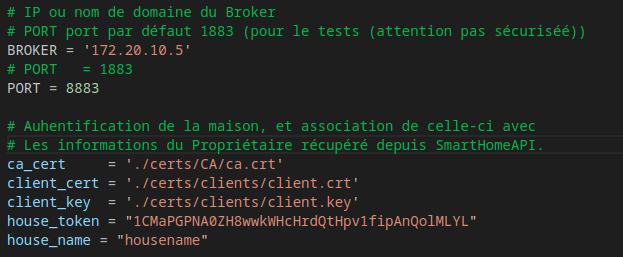
\includegraphics[width=0.75\textwidth]{ressources/img/preuves/champsRenseignes}
			\caption{Champs à renseigner au sein de \textbf{HomeSimulation : main.py}}
			\label{fig:champsARenseigner}
		\end{figure}
		
		\begin{figure}[h!]
			\centering
			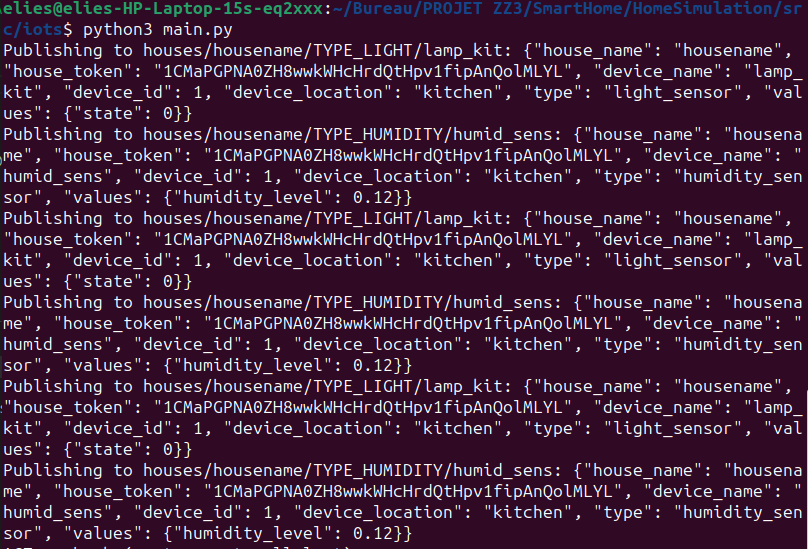
\includegraphics[width=0.75\textwidth]{ressources/img/preuves/envoieDonnesAPI}
			\caption{Envoie de 2 séries de données au serveur: \textbf{172.20.10.5}}
			\label{fig:envoieDonnees}
		\end{figure}
		Ainsi, les données sont envoyées à \textbf{Mosquitto}, et stockés dans \textbf{InfluxDB}.
	\paragraph{Accès aux données des capteurs via SmartHouseAPI à temps réel}
	Une fois les données \textbf{envoyées} et \textbf{stockées dans InfluxDB}, il est nécessaire de \textbf{vérifier leur accessibilité via SmartHouseAPI}. Par le biais du \textbf{token unique attribué lors de l’enregistrement de la maison}, seul le propriétaire peut récupérer les données associées à ses capteurs.\\
	
	L’accès aux données s’effectue en envoyant une requête \textbf{GET} à l’API, en fournissant \textbf{le token en paramètre}. L’API interroge alors \textbf{InfluxDB} pour \textbf{extraire les séries de données correspondant à la maison demandée}.\\\\
	
	\textbf{Récupération de la dernière données acquise}
	\begin{figure}[h!]
		\centering
		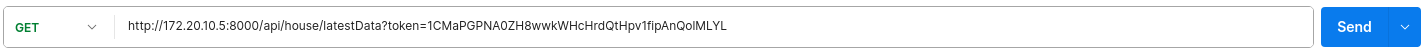
\includegraphics[width=1\textwidth]{ressources/img/preuves/lastDataRequete}
		\caption{Requête de récupération de la \textbf{dernière donnée acquise}}
		\label{fig:lastDataRequete}
	\end{figure}
	\newpage
	\begin{figure}[h!]
		\centering
		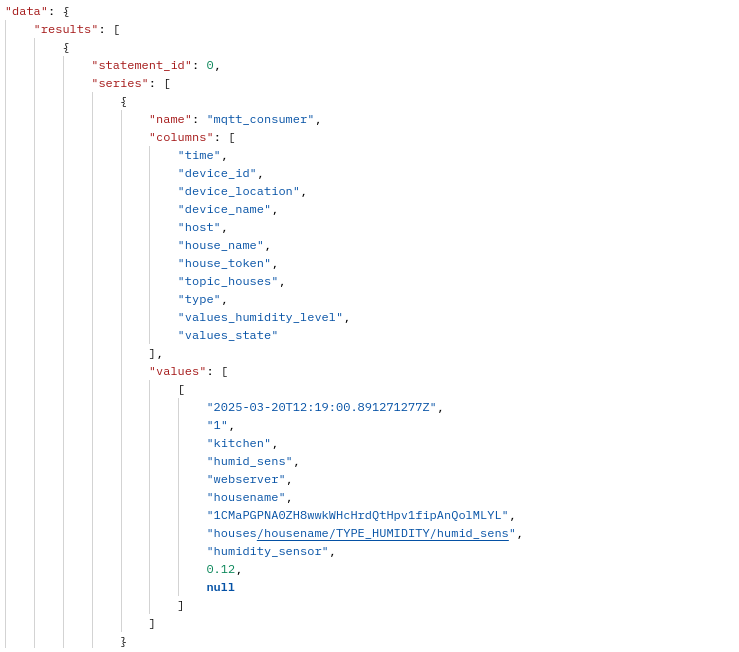
\includegraphics[width=0.75\textwidth]{ressources/img/preuves/lastDataReponse}
		\caption{Réponse de l'API de la dernière données acquise}
		\label{fig:lastDataReponse}
	\end{figure}
	\vspace{1cm}
	\textbf{Récupération de données filtrées en fonction du capteur d'humidité}
	\begin{figure}[h!]
		\centering
		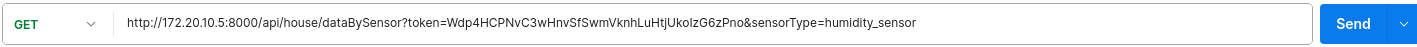
\includegraphics[width=1\textwidth]{ressources/img/preuves/dataBySensorRequete}
		\caption{Requête de récupération des \textbf{données acquises par capteur d'humidité}}
		\label{fig:dataBySensorRequete}
	\end{figure}
	\newpage
	\begin{figure}[h!]
		\centering
		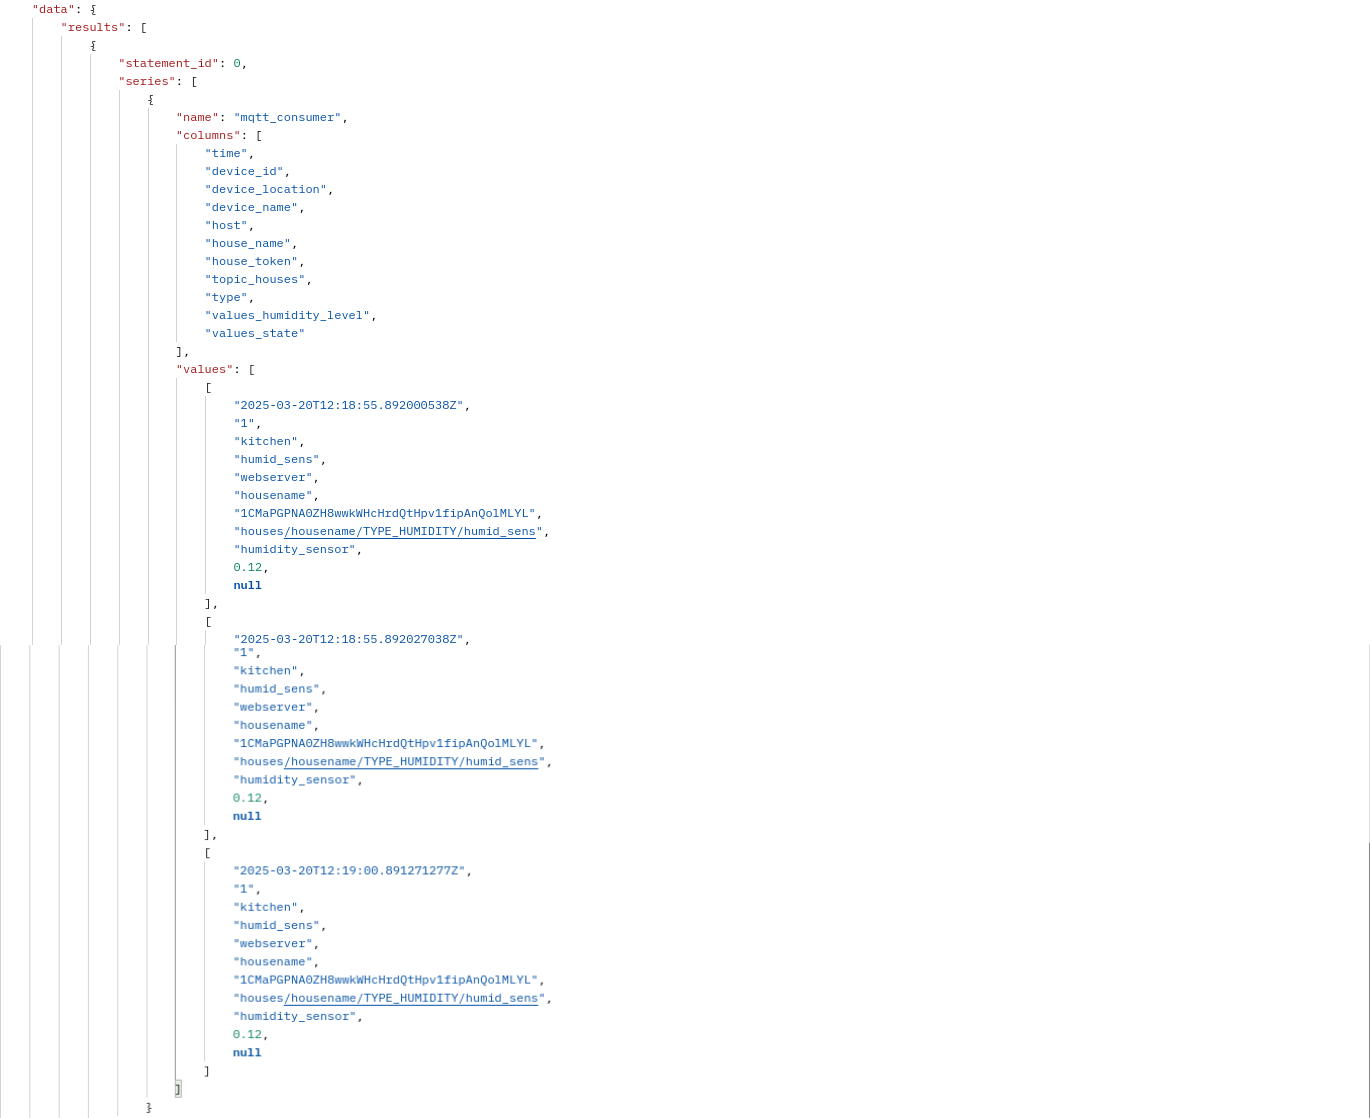
\includegraphics[width=0.75\textwidth]{ressources/img/preuves/dataBySensorReponse}
		\caption{Réponse de l'API des \textbf{données acquises par capteur d'humidité}}
		\label{fig:dataBySensorResponse}
	\end{figure}
	
	\paragraph{Synthèse des Tests}
	Les tests effectués confirment \textbf{le bon fonctionnement de SmartHouseAPI}, démontrant que l’architecture mise en place\textbf{ répond aux exigences définies}. L’authentification des maisons via les certificats \textbf{SSL/TLS} et les \textbf{tokens} uniques s'est révélée efficace, \textbf{garantissant un accès sécurisé aux données}.
	
	Les requêtes envoyées via \textbf{Postman} ont permis de \textbf{valider les différentes fonctionnalités de l’API}, notamment la \textbf{création d’un propriétaire}, l’\textbf{association des certificats}, et l’\textbf{accès aux données stockées dans InfluxDB}. L'\textbf{API} a correctement \textbf{filtré} et \textbf{renvoyé} les \textbf{informations des capteurs en fonction des permissions définies, confirmant ainsi son rôle central dans la gestion et la sécurisation des échanges}.
	
	Ces résultats démontrent que l’\textbf{API} fonctionne \textbf{comme prévu}, offrant un \textbf{accès structuré}, \textbf{fiable} et\textbf{ sécurisé aux données des maisons connectées}.\newpage
	
	\section{Surveillance des données avec une interface graphique}
	L’\textbf{intégration d’une interface graphique} est un \textbf{élément clé} dans la \textbf{gestion} et la \textbf{surveillance d’un système de maison connectée}. Une interface utilisateur intuitive permet aux propriétaires de \textbf{visualiser en temps réel l’état de leurs capteurs}, d’interpréter rapidement les données collectées et d’interagir avec le système. Sans cette couche visuelle, l’exploitation des informations se limiterait à des \textbf{requêtes API} et des \textbf{réponses JSON}, ce qui serait\textbf{ peu convivial pour un utilisateur non technique}.\\
	
	Pour le développement de cette interface, nous avons choisi \textbf{QT}, un \textbf{framework puissant} et \textbf{énormément utilisé pour la création d’applications multiplateformes en C++}. \textbf{QT} offre plusieurs avantages qui en font un outil performant pour notre projet :
	
	\begin{itemize}
		\item \textbf{Simplicité de gestion de la mémoire: } Contrairement à un programme \textbf{C++ classique} où il est nécessaire de gérer la création ainsi que la \textbf{destruction des objets}, QT \textbf{réduit les risques de fuites de mémoire} en assurant une \textbf{gestion optimisée des ressources en mémoire}.
		
		\item \textbf{Documentation et support communautaire:}  \textbf{QT} bénéficie d’une documentation complète et largement accessible, ce qui \textbf{facilite la prise en main} et l’\textbf{implémentation des divers fonctionnalités fournies par le framework}. 
		
		\item \textbf{Compatibilité multiplateforme :} Une application développée avec \textbf{QT} peut être exécutée sur\textbf{ Windows, Linux, macOS et même certaines plateformes embarquées}, offrant ainsi une praticité accrue pour le déploiement.
		\item \textbf{Intégration avec l’API REST :} \textbf{QT} permet une\textbf{ gestion efficace des requêtes réseau}, ce qui permet de \textbf{récupérer les données en temps réel depuis SmartHouseAPI}, de les \textbf{traiter} et de les \textbf{afficher} sous \textbf{forme de graphiques interactifs pour une meilleure surveillance des données issus des capteurs}.
	\end{itemize}
	\vspace{0.5cm}
	Grâce à \textbf{QT}, nous avons pu développer un début d’interface permettant de \textbf{récupérer} et \textbf{parser} les données \textbf{issues de l’API}. Bien que l’affichage graphique n’ait pas encore été finalisé, cette première implémentation pose \textbf{les bases d’un système de monitoring}, ouvrant la voie à des \textbf{améliorations futures telles que l’ajout de tableaux de bord dynamiques et d’un contrôle interactif des équipements connectés}.
	
	\subsection{Architecture logicielle de l'application SmartHouse Monitoring}	
	
	\paragraph{Structure de SmartHouse Monitoring}
		Tout d'abord, il est \textbf{essentiel de comprendre la structure d’un projet Qt en C++}. Un projet Qt repose sur un fichier \textbf{.pro}, qui définit sa \textbf{configuration}, les \textbf{bibliothèques utilisées} ainsi que les \textbf{paramètres de compilation}. Il est composé de \textbf{fichiers source} et \textbf{en-têtes}, qui contiennent respectivement l’\textbf{implémentation} ainsi que la \textbf{définition des classes}. L’interface graphique peut être \textbf{conçue à l’aide de fichiers .ui, générés via Qt Designer}, mais dans notre cas, nous avons préféré structurer l’interface directement depuis le code, en créant des classes dédiées afin d'avoir un contrôle plus précis sur l’affichage. Enfin, un projet peut inclure des fichiers de ressources (.qrc), permettant d’intégrer des éléments tels que des \textbf{icônes} et \textbf{images} nécessaires à l'affichage.\\\\
		Ainsi, le développement de \textbf{SmartHouse Monitoring} s'est structuré autour de cette architecture en commençant par la \textbf{configuration du projet QT} via le fichier \textbf{.pro}. Cette étape a permis d’intégrer les bibliothèques essentielles au bon fonctionnement de l’application. Tout d’abord, l’ajout des \textbf{bibliothèques réseau (QtNetwork)} a été nécessaire afin de permettre l’envoi et la réception de requêtes HTTP, assurant ainsi la communication avec \textbf{SmartHouseAPI} pour récupérer les données des capteurs en temps réel. Ensuite, l’utilisation des\textbf{ widgets (QtWidgets)} a facilité la conception de l’interface utilisateur, en offrant des composants interactifs tels que \textbf{fenêtres}, \textbf{boutons} et \textbf{champs de saisie}, rendant l’application \textbf{ergonomique} et \textbf{intuitive}. Enfin, l’intégration des bibliothèques \textbf{graphiques (QtCharts)} dans le but d'afficher des \textbf{courbes} et des \textbf{graphiques dynamiques}, afin d'offrir une visualisation \textbf{claire} et \textbf{efficace} des données capturées par les capteurs IoT.
		
	\paragraph{Explication des différentes classes de SmartHouse Monitoring}
	
	\begin{figure}[h!]
		\centering
		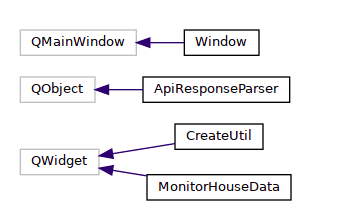
\includegraphics[width=0.75\textwidth]{ressources/img/shémas/hierarchieQT.png}
		\caption{Architecture des classes de \textbf{SmartHouse Monitoring}}
		\label{fig:hierarchieQT}
	\end{figure}
	
	
	\chapter{Résultats et Discussion}
	À l’issue de ce projet, nous avons pu mettre en place un système de surveillance des données issues de maisons connectée, sécurisé. l'architecture globale intègre plusieurs technologies, assurant l'\textbf{émission} et la \textbf{réception} des données en temps réel via le protocole MQTTs, ainsi que leur \textbf{stockage} et leur \textbf{affichage}.\\
	\section{Situation à la fin de l’étude}

	En l'absence de dispositifs physiques, nous avons développé \textbf{HomeSimulation}, un \textbf{simulateur en Python}, exécuté sur l’une de nos machines, afin de reproduire le comportement de capteurs IoT. Cette simulation permet de \textbf{créer une ou plusieurs maisons virtuelles} capables d’émettre, via le protocole MQTTs, des séries de données générées aléatoirement, \textbf{simulant ainsi les mesures des capteurs connectés}.\\
	L’architecture de la simulation a été conçue pour être \textbf{extensible}, facilitant l’ajout de nouveaux dispositifs et ne limitant ni le \textbf{nombre de capteurs} présents dans une maison ni la \textbf{fréquence d’envoi} des données.\\
	Cette approche permet de \textbf{tester} et \textbf{valider} l’ensemble du système dans des conditions \textbf{proches d’une utilisation réelle}, permettant ainsi la simulation divers scénarios d’exploitation sans nécessiter de matériel physique.\\
	
	La transmission des données générées par \textbf{HomeSimulation} vers la base de données est assurée via \textbf{Mosquitto}, un \textbf{broker MQTT} reconnu pour sa \textbf{légèreté} et sa \textbf{fiabilité}. Afin de garantir la sécurité des échanges, nous avons mis en place une authentification basée sur \textbf{SSL/TLS}, assurant ainsi que \textbf{seules les maisons autorisées peuvent communiquer avec le serveur}. Ce protocole permet de \textbf{chiffrer les données en transit}, les protégeant contre \textbf{toute interception} ou \textbf{modification malveillante}. Cette sécurisation est essentielle dans le cadre d’un système de maison connectée, où la \textbf{confidentialité} et l’\textbf{intégrité} des informations transmises sont essentiels.\\
	
	\textbf{SmartHomeAPI}, l'\textbf{API REST} que nous avons développée en PHP avec le framework \textbf{Laravel} constitue \textbf{le cœur de notre architecture}. Elle permet d'\textbf{authentifier} les propriétaires des maisons connectées, de \textbf{générer des certificats SSL} et de récupérer les \textbf{données stockées via InfluxDB}, en utilisant un token d'authentification, unique à chaque utilisateur. L'\textbf{API} a été conçue de manière à être totalement \textbf{indépendante} de l'interface utilisateur, ce qui la rend \textbf{utilisable} avec tout type d'interface future – qu'il s'agisse d'une \textbf{application web}, d'\textbf{une application Android} ou \textbf{iOS}. Cette modularité garantit que l’API n’aura pas besoin d'être modifiée en cas d’évolution des supports ou des interfaces, assurant ainsi une grande \textbf{pérennité} et \textbf{évolutivité} pour l'ensemble du système.\\
	
	Pour l’interface utilisateur, nous avons opté pour \textbf{Qt}, une technologie très utilisée en entreprise et en industrie, nous permettant ainsi \textbf{d’approfondir nos compétences en développement C++}, et de l'utiliser dans un but plus tangible. Ce choix nous a offert une approche plus concrète du développement d’interfaces graphiques et de leur interaction avec une API REST.	
	Grâce à Qt, nous avons pu \textbf{récupérer} et \textbf{parser} les données issues de la maison connectée, établissant ainsi une \textbf{base solide pour la visualisation des informations en temps réel}. Toutefois, la dernière étape, qui consistait à \textbf{afficher ces données sous forme de graphiques dynamiques et interactifs}, n’a pas pu être finalisée par manque de temps.
	Malgré cela, cette phase nous a permis de mieux appréhender l’intégration de Qt avec notre \textbf{API REST}, en posant les \textbf{fondations nécessaires pour d’éventuelles améliorations}. À terme, cette interface pourrait être enrichie avec des fonctionnalités d’analyse visuelle avancées, permettant une surveillance optimisée des équipements connectés.
	
	\section{Analyse des résultats obtenus}
	
	Lors de l’analyse des résultats, nous avons mené une\textbf{ série de tests} visant à \textbf{optimiser la structuration des topics MQTT} et à \textbf{déterminer le format de données le plus adapté à la simulation des capteurs.}
	
	Dans un premier temps, nous avons réalisé \textbf{des tests de transmission de données} en \textbf{clair}, afin d’analyser la \textbf{fluidité} et la \textbf{fiabilité} des échanges. Par la suite, nous avons sécurisé la communication en \textbf{activant MQTTs} et en \textbf{intégrant des certificats SSL}, garantissant ainsi l’\textbf{authentification} et le \textbf{chiffrement des échanges}.
	
	Ces expérimentations nous ont permis d’évaluer la \textbf{robustesse} du protocole et d\textbf{’analyser l'impact de la sécurisation sur les performances globales du système}, notamment en termes de \textbf{latence}.
	
	Les tests effectués ont confirmé plusieurs points forts de notre système : 
	\begin{itemize}
		\item  \textbf{Sécurisation des données :} La transmission est sécurisée grâce à l'utilisation de MQTTs combiné aux \textbf{certificats SSL/TLS}, garantissant ainsi un \textbf{chiffrement complet} et \textbf{protégeant les échanges contre toute tentative d'interception}.  
		\item  \textbf{Efficacité de l’API REST :} L’\textbf{API REST}, remplit \textbf{efficacement son rôle d'intermédiaire} en \textbf{filtrant} et en fournissant les données requises par les maisons connectées, assurant ainsi une communication \textbf{fluide} entre les différents composants du système.  
		\item  \textbf{Intégration avec InfluxDB :} La base de données InfluxDB permet une \textbf{récupération rapide} et optimisée des \textbf{données historiques} ainsi que des\textbf{ données en temps réel}, ce qui est essentiel pour une \textbf{réponse réactive de l'API}.  
		\item  \textbf{Authentification par certificat :} Le mécanisme d'authentification par certificat, des maisons renforce la sécurité en garantissant que seules les maisons \textbf{préalablement enregistrées peuvent communiquer avec le serveur, limitant ainsi les risques d'intrusion.}
	\end{itemize} 


	
	\chapter{Conclusion}
	Ce projet nous a permis d’explorer et de mettre en œuvre plusieurs technologies essentielles à la domotique et à l’Internet des objets (IoT). Dès le début, nous avons conçu un système de communication sécurisé permettant l’échange en temps réel des données entre une maison connectée et un serveur central. Cette communication constitue la base indispensable pour assurer un suivi fiable des équipements et optimiser leur gestion.
	
	La sécurisation des échanges a été une priorité majeure, avec l’intégration de MQTTs et de certificats SSL/TLS garantissant l’authenticité des émetteurs et l’intégrité des données transmises. De plus, le choix de InfluxDB pour le stockage des données temporelles a permis d’assurer une récupération rapide et efficace des informations, tout en facilitant l’analyse des historiques.
	
	L’API REST développée sous Laravel joue un rôle clé en assurant une interface sécurisée et modulaire entre les équipements IoT et les systèmes clients. Son architecture indépendante de toute interface utilisateur permet une compatibilité future avec divers supports, qu’il s’agisse d’applications web, Android ou iOS.
	
	Enfin, bien que l’interface utilisateur en Qt ne soit pas totalement finalisée, les bases sont bien établies. Nous avons pu récupérer et parser les données depuis l’API, ouvrant la voie à une intégration future de visualisations graphiques dynamiques. Cette expérience nous a permis d’approfondir nos connaissances en C++, tout en renforçant notre compréhension des interactions entre une interface graphique et une API REST.\\
	
	\paragraph{Réponse à la problématique}
	\textbf{\textit{Comment développer un système de monitoring en temps réel pour une maison connectée, garantissant la sécurité de la transmission des données tout en renforçant l'authentification des équipements IoT ?}}\vspace{1cm}
	
	Ce projet apporte une \textbf{réponse concrète et fonctionnelle à cette problématique}. Grâce à l’utilisation de \textbf{MQTTs}, nous avons mis en place un \textbf{canal de communication sécurisé garantissant l’authenticité des équipements et la confidentialité des échanges} par le biais de certificats \textbf{SSL/TLS}, limitant \textbf{l’accès aux seules maisons enregistrées}.
	
	De plus, l’\textbf{API REST} centralisée permet de \textbf{filtrer} et récupérer les \textbf{données IoT}, tout en offrant une architecture extensible et adaptable. Enfin, l’implémentation de \textbf{InfluxDB} permet de gérer efficacement les données en \textbf{temps réel}, garantissant une \textbf{réactivité optimale du système}.
	
	En conclusion, notre projet répond aux exigences de \textbf{sécurité} et de \textbf{surveillance en temps réel} pour une maison connectée, tout en offrant une base évolutive permettant d’enrichir et d’améliorer ses fonctionnalités dans le futur.
	
	\section{Limites et améliorations possibles}
	
	Malgré des bases solides, il est toujours possible \textbf{d’envisager des améliorations afin d’approcher encore davantage notre projet de la réalité et de renforcer sa sécurité}. En effet, bien que notre système dispose d\textbf{’un premier niveau de sécurité complet}, nous aurions pu aller plus loin dans la réflexion sécuritaire, notamment en développant notre API pour qu’\textbf{elle fonctionne en HTTPS plutôt qu’en HTTP}. Cela aurait permis d’assurer une transmission entièrement \textbf{chiffrée} des requêtes, garantissant ainsi une protection accrue des données en transit et une meilleure adaptation aux exigences de sécurité du monde réel.
	
	Sur le plan de l’interface, des améliorations auraient également pu être apportées \textbf{pour renforcer la connexion utilisateur}. Actuellement, l’authentification repose sur un \textbf{mécanisme à facteur unique (1FA)} utilisant uniquement un \textbf{token}. La mise en place d’un\textbf{ second facteur d’authentification}, ou encore \textbf{l’implémentation d’un système reposant sur OAuth2}, aurait permis d’offrir une sécurité renforcée pour \textbf{les comptes utilisateurs et de réduire le risque d’accès non autorisé}.
	
	Concernant l’interface graphique, nous avons choisi de ne pas utiliser d’outil déjà existant, tel que \textbf{Grafana}, afin de nous \textbf{perfectionner dans la compréhension et l’utilisation de Qt}, et d'utiliser le language C++ à \textbf{des fins plus concrètes}. Cette décision nous a demandé un effort supplémentaire, puisque nous avons dû développer nous-mêmes une interface qui, bien qu’elle ne soit pas finalisée, démontre déjà notre capacité à \textbf{récupérer} et \textbf{parser} les données via l’\textbf{API REST}. Une alternative aurait été d’implémenter d’abord \textbf{Grafana} pour disposer rapidement d’un \textbf{outil de visualisation efficace, puis d’envisager par la suite soit de l’utiliser tel quel, soit de développer un outil personnalisé plus complet et intuitif pour afficher les données en temps réel}. Cela nous aurait permis d’obtenir dès le départ un aperçu précis des données utilisateur, même si dans notre cas il s’agissait de données simulées.
	
	Enfin, pour se rapprocher encore plus d’un environnement de production, il aurait été intéressant de déployer \textbf{notre projet sur un serveur réellement distant}, par exemple en utilisant des services de CLOUDS tels qu’\textbf{Azure} ou \textbf{AWS}. Ce déploiement aurait permis de mettre en réseau notre application et de la rendre accessible depuis \textbf{n’importe quel appareil possédant un compte utilisateur, ouvrant ainsi la voie à une utilisation à plus grande échelle}. 
	
	Toutefois, en dépit de ces limites mineures et corrigeables, ce projet a été une expérience enrichissante, permettant d’\textbf{explorer} et d’\textbf{approfondir} des concepts essentiels en \textbf{réseau}, \textbf{sécurité} et \textbf{développement IoT}.	
	
	\appendix
	\chapter{Annexes}
	\section{Lexique}
	\section{Bibliographie}
	\section{Webographie}
	
	
	
		
	
	\nocite{*}
	\bibliographystyle{unsrt}
	\bibliography{references}
	
	\clearpage
	
	\printglossaries
	
	
\end{document}